\documentclass[12pt,a4paper,bibtotoc]{scrartcl}

\usepackage[sc]{mathpazo}
\usepackage[onehalfspacing]{setspace}
\usepackage[T1]{fontenc}
\usepackage[utf8]{inputenc}
\usepackage[ngerman]{babel}
\usepackage{geometry}
\usepackage{amsmath}
\usepackage{amsfonts}
\usepackage{amssymb}
\usepackage{graphicx}
\usepackage{natbib}
\usepackage[hyphens]{url}
\usepackage[printonlyused, withpage]{acronym}
\usepackage{listings}
\usepackage{color}
\usepackage{beramono}
\usepackage{wrapfig}
\usepackage{pdfpages}
%\usepackage{hyperref}

\geometry{a4paper, portrait, left=2.5cm, right=2.5cm, top=2cm, bottom=2cm}
\parindent0cm

\pagestyle{headings}

\author{Malte Modrow}

\definecolor{lightgray}{rgb}{.9,.9,.9}
\definecolor{darkgray}{rgb}{.4,.4,.4}
\definecolor{purple}{rgb}{0.65, 0.12, 0.82}

\definecolor{gray}{rgb}{0.4,0.4,0.4}
\definecolor{darkblue}{rgb}{0.0,0.0,0.6}
\definecolor{cyan}{rgb}{0.0,0.6,0.6}

\lstdefinelanguage{JavaScript}{
  keywords={typeof, new, true, false, catch, function, return, null, catch, switch, var, if, in, while, do, else, case, break},
  keywordstyle=\color{blue}\bfseries,
  ndkeywords={class, export, boolean, throw, implements, import, this},
  ndkeywordstyle=\color{darkgray}\bfseries,
  identifierstyle=\color{black},
  sensitive=false,
  comment=[l]{//},
  morecomment=[s]{/*}{*/},
  commentstyle=\color{purple}\ttfamily,
  stringstyle=\color{red}\ttfamily,
  morestring=[b]',
  morestring=[b]"
}

\lstdefinelanguage{XML}{
	morestring=[b]",
  	morestring=[s]{>}{<},
  	morecomment=[s]{<?}{?>},
  	stringstyle=\color{black},
  	identifierstyle=\color{darkblue},
  	keywordstyle=\color{cyan},
  	morekeywords={xmlns,version,type}
}

\lstset{
   backgroundcolor=\color{lightgray},
   extendedchars=true,
   basicstyle=\footnotesize\ttfamily,
   columns=flexible,
   frame=single,
   showstringspaces=false,
   showspaces=false,
   numbers=left,
   numberstyle=\footnotesize,
   numbersep=9pt,
   tabsize=4,
   breaklines=true,
   showtabs=false,
   captionpos=b,
   escapechar=',
   inputencoding=utf8,
   belowskip=2em,
   aboveskip=3em,
   literate={Ö}{{\"O}}1{Ä}{{\"A}}1{Ü}{{\"U}}1{ß}{{\ss}}2{ü}{{\"u}}1{ä}{{\"a}}1{ö}{{\"o}}1{©}{{\copyright}}1
}


\begin{document}
%\clearpage\pdfbookmark{\contentsname}{toc}\tableofcontents
\thispagestyle{plain}
\tableofcontents
\thispagestyle{plain}

\newpage
\listoffigures
\vspace{2cm}
\listoftables

\newpage
\lstlistoflistings
\vspace{2cm}
\section*{Abkürzungsverzeichnis}
\label{sec:abkürzungen}
\begin{acronym}[SEPSEP]
	\acro{xaml}[XAML]{Extensible Application Markup Language}
	\acro{cms} [CMS]{Content Management System}
	\acro{xml} [XML]{Extensible Markup Language}
	\acro{xslt}[XSLT]{Extensible Stylesheet Language Transformations}
	\acro{html}[HTML]{Hypertext Markup Language}
	\acro{xhr}[XHR]{XMLHttpRequest}
	\acro{winjs}[WinJS] {Windows Library for JavaScript}
\end{acronym}

\newpage
\section{Einleitung}
\label{sec:einleitung}
\newpage
\section{Windows 8}
\label{sec:windows8}
Seit dem 26. Oktober 2012 ist Microsofts aktuellstes Betriebssystem \glqq Windows 8\grqq\ für die breite Öffentlichkeit verfügbar. Dieses unterscheidet sich grundlegend von seinem Vorgänger \glqq Windows 7\grqq. Microsoft verfolgt mit Windows 8 den Ansatz, das gleiche Betriebssystem sowohl für Desktop- als auch für Tablet-Computer\footnote{Tablet-Computer: kleiner, flacher, tragbarer Computer mit einem Touchscreen. Es wird von nun an, der Einfachheit halber die englische Version \glqq Tablet\grqq\ benutzt.} zu verwenden. Es besitzt nach wie vor den bekannten Desktop von Windows 7. Äußerlich sind hier nur kleine Änderungen vorgenommen worden. So besitzt z.B. der Windows Explorer eine neues, kontextsensitives Ribbon-Menü\footnote{Auch bekannt als Menüband oder Multifunktionsleiste.}. Neu ist hingegen das "Modern User Interface" (Modern UI, früher Metro), eine für Touch-Gesten optimierte Oberfläche. Obwohl die neue Oberfläche für Touch-Gesten optimiert ist, kann sie ebenso mit Maus und Tastatur bedient werden. Es können, im Gegensatz zum Desktop, keine herkömmlichen Programme im Modern UI ausgeführt werden. In der Modern UI Oberfläche laufen nur Programme (Apps), die speziell für Windows 8 entwickelt wurden und über den Microsoft Store (siehe Sektion \ref{subsubsec:store} auf Seite \pageref{subsubsec:store}) erhältlich sind. Es soll nun ein etwas detaillierterer Blick auf die neue Oberfläche und dessen Eigenheiten geworfen werden.

\subsection{Neues Bedienkonzept}
\label{subsec:bedienkonzept}
Beim Hochfahren von Windows 8, erwartet den User ein Interface, das er so vom Vorgänger Windows 7 nicht kennt. Viele bunte, viereckige Kacheln, in verschiedenen Größen. So sieht die neue Startoberfläche von Windows 8 aus (siehe Abbildung \ref{fig:win8startscreen}). Auf dem Startbildschirm sind die verschiedenen Programme angeordnet.

\begin{figure}[h]	
	\centering
	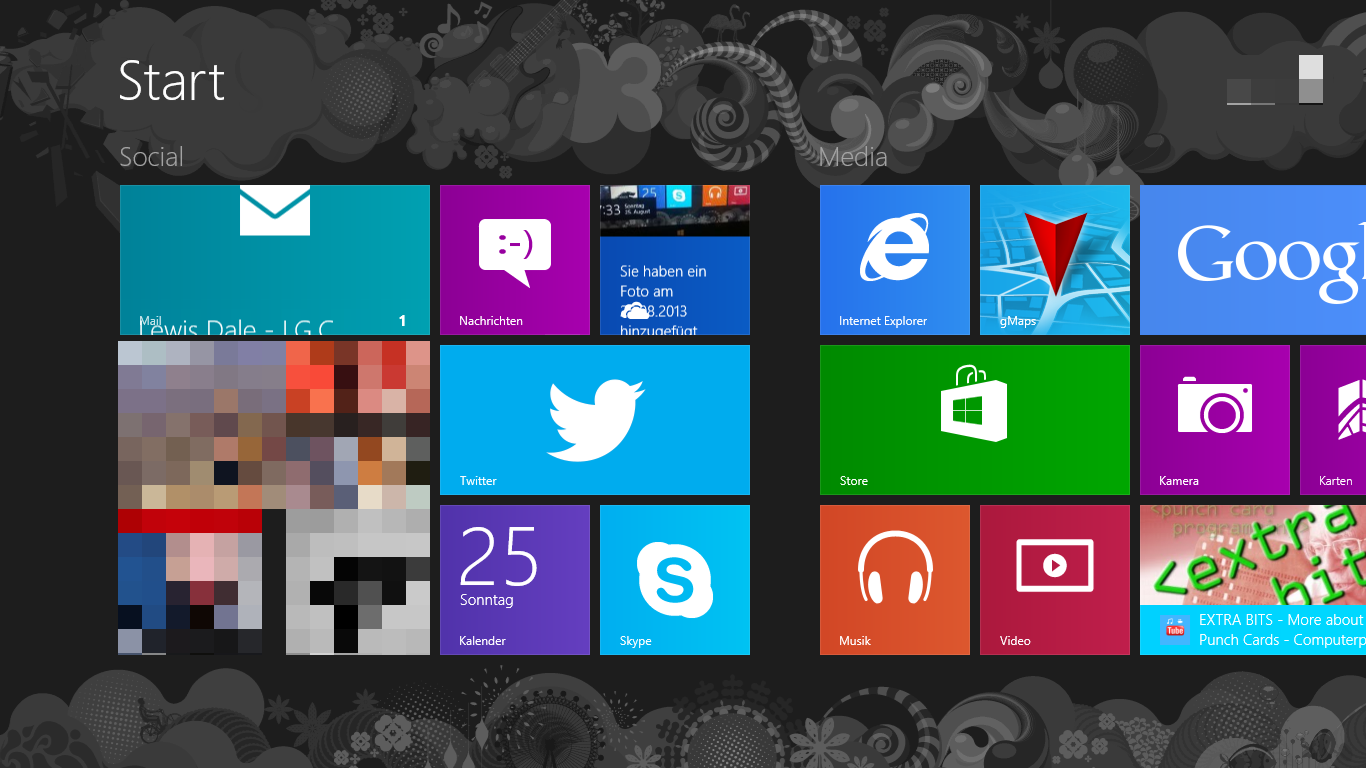
\includegraphics[width=0.6\textwidth]{Bilder/Screenshots/windows8/win8_startscreen.png} 
	\caption{Der Startbildschirm von Windows 8.}
	\label{fig:win8startscreen}
\end{figure}

Dies können \glqq normale\grqq\ Programme sein, die auf dem Desktop laufen oder es können Modern UI Apps (Windows-Store) sein, welche nur über den Microsoft Store zu installieren sind. Der bekannte Desktop-Modus ist in diesem Sinne auch \glqq nur\grqq\ ein, wenn auch ein sehr spezielles, Programm (App), welches in der neuen Oberfläche gestartet und ausgeführt werden kann.\\
Es gibt einige grundlegende Touch- und Mausgesten um in der Modern UI Oberfläche zwischen den Apps zu navigieren oder um Optionen oder Einstellungen aufzurufen. Wenn der User sich auf einem Tablet befindet und über den rechten Bildschirmrand von rechts nach links wischt (swipen), öffnet sich am rechten Bildschirmrand die von Microsoft \glqq Charms\grqq\ genannte Menüleiste (siehe Abbildung \ref{fig:charms}. Hier befinden sich die Schaltflächen: Suchen, Teilen, \glqq zur Startansicht\grqq\ , Geräte und Einstellungen. Um die Charms-Bar auf einem Gerät ohne Touch-Unterstützung aufzurufen, muss die Maus in die obere oder untere rechte Ecke des Bildschirms geführt werden. 

\begin{figure}[h]	
	\centering
	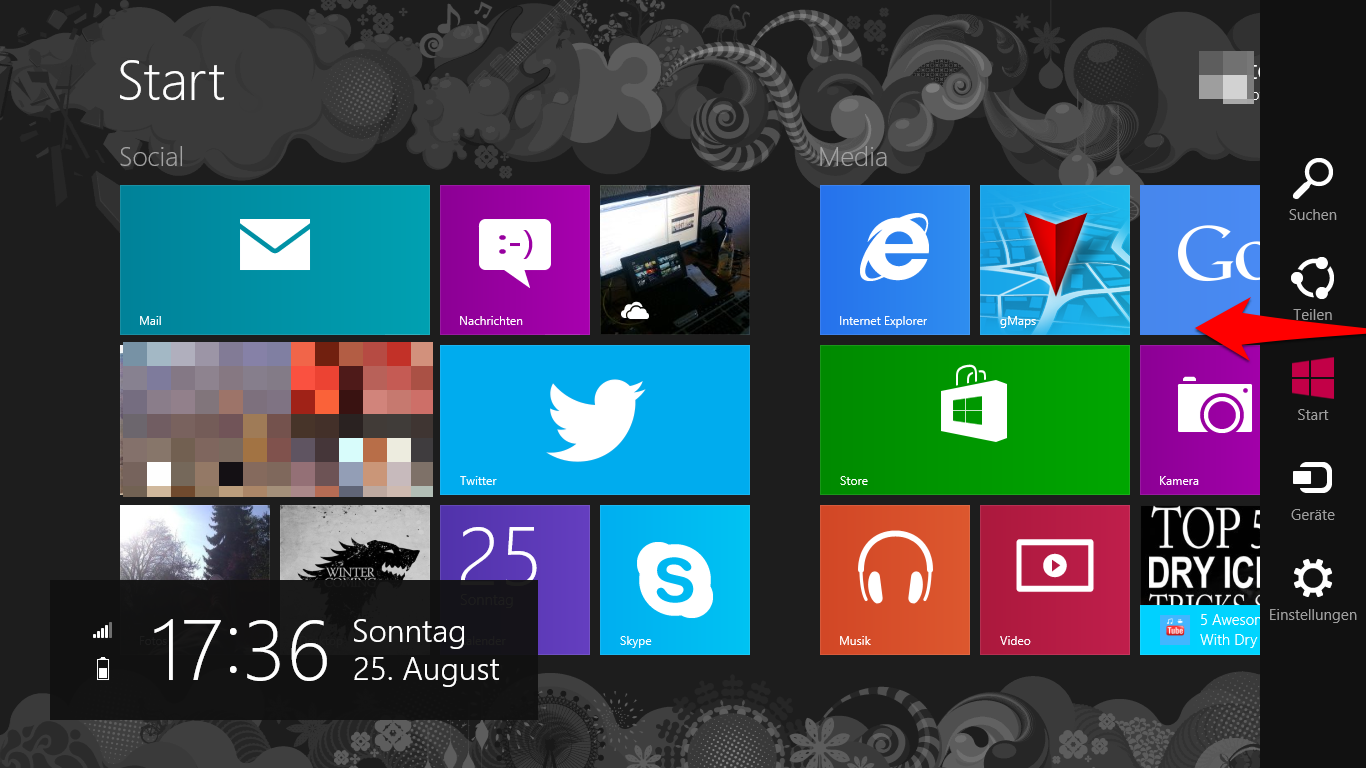
\includegraphics[width=0.6\textwidth]{Bilder/Screenshots/windows8/charm_bar.png} 
	\caption{Die Geste zum Aufrufen der Charms-Menüleiste.}
	\label{fig:charms}
\end{figure}  

Um bequem zwischen den geöffneten Apps zu wechseln, können zwei verschiedene Gesten benutzt werden. Abbildung \ref{fig:appschanging} zeigt die beiden Möglichkeiten. Um eine Liste wie sie die Abbildung auf der linken Seite zeigt angezeigt zu bekommen, wird von links nach rechts über den linken Bildschirmrand gewischt. Anschließend wird ohne den Finger hochzunehmen zurück in Richtung des Bildschirmrandes gewischt. Bei der Bedienung mit der Maus, wird die Maus zunächst in die obere oder untere linke Ecke bewegt, um anschließend runter bzw. hoch zur Bildschirmmitte geführt zu werden.\\
Die zweite Möglichkeit besteht darin, die Apps direkt in der Reihenfolge wie sie zuletzt aktiv waren wieder in den Vordergrund zu bringen. Dazu wird von links nach rechts über den linken Bildschirmrand gewischt. Der rechte Teil von Abbildung \ref{fig:appschanging} zeigt diese Geste.
 
\begin{figure}[h]	
	\centering
	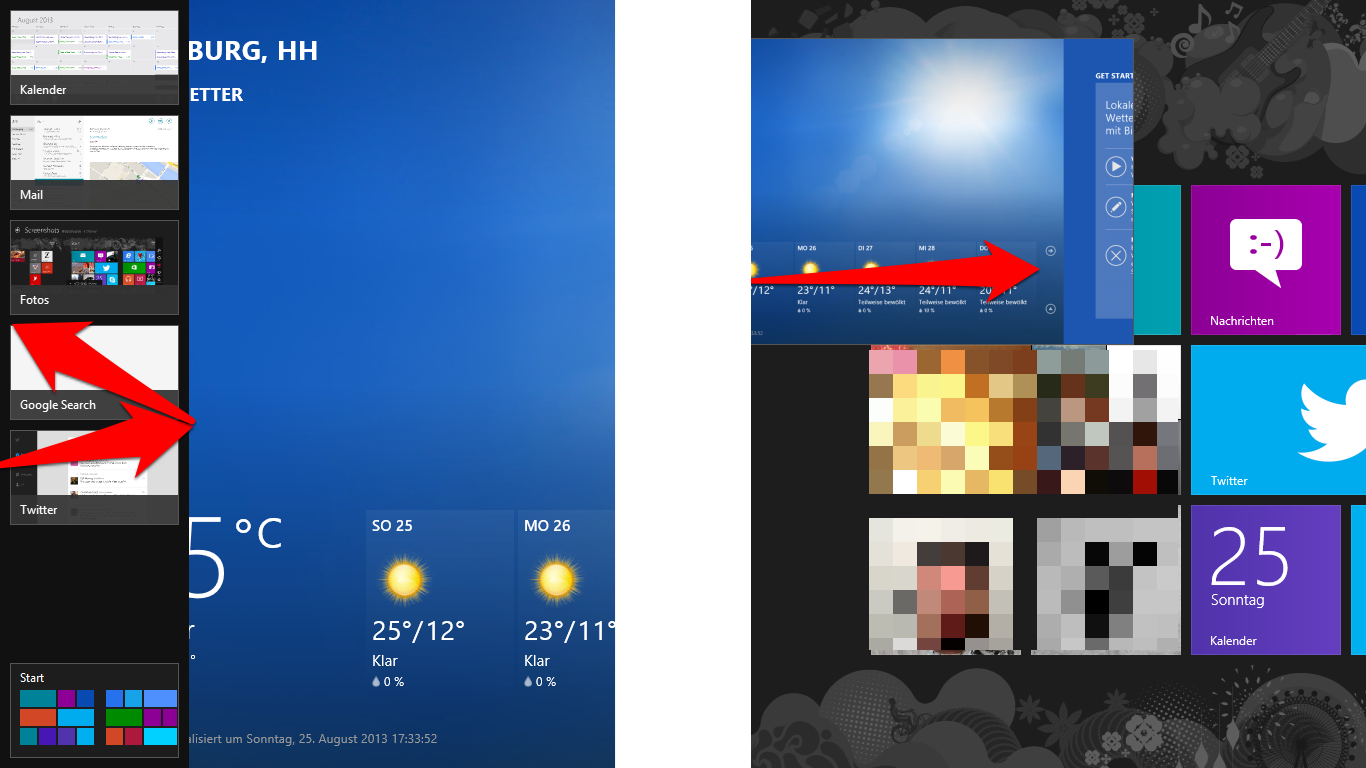
\includegraphics[width=0.6\textwidth]{Bilder/Screenshots/windows8/apps_changing.png} 
	\caption{Die Gesten zum Durch-wechseln der Apps.}
	\label{fig:appschanging}
\end{figure}  

Die letzte grundlegende Geste, wird benutzt um z.B. Optionen, Einstellungen oder eine Navigationsleiste aufzurufen. Hierzu wird über den oberen oder den unteren Bildschirmrand in Richtung Bildschirmmitte gewischt. Wird diese Geste ausgeführt öffnen sich die untere und die obere Menüleiste. Es ist egal ob der User die Geste am oberen oder am unteren Bildrand ausführt. Wenn es in der App oben und unten Menüleisten gibt, öffnen sich immer beide. Es ist nicht möglich z.B. nur die obere Leiste zu öffnen. In der unteren Menüleiste befinden sich typischer Weise Einstellungen für die aktuelle Ansicht, in welcher sich die App gerade befindet. In der oberen Leiste ist typischer Weise eine Art von Navigation untergebracht (falls es eine obere Leiste gibt). Abbildung \ref{fig:menubar} zeigt die obere und untere Menüleisten am Beispiel der vorinstallierten Wetter App.

\begin{figure}[h]	
	\centering
	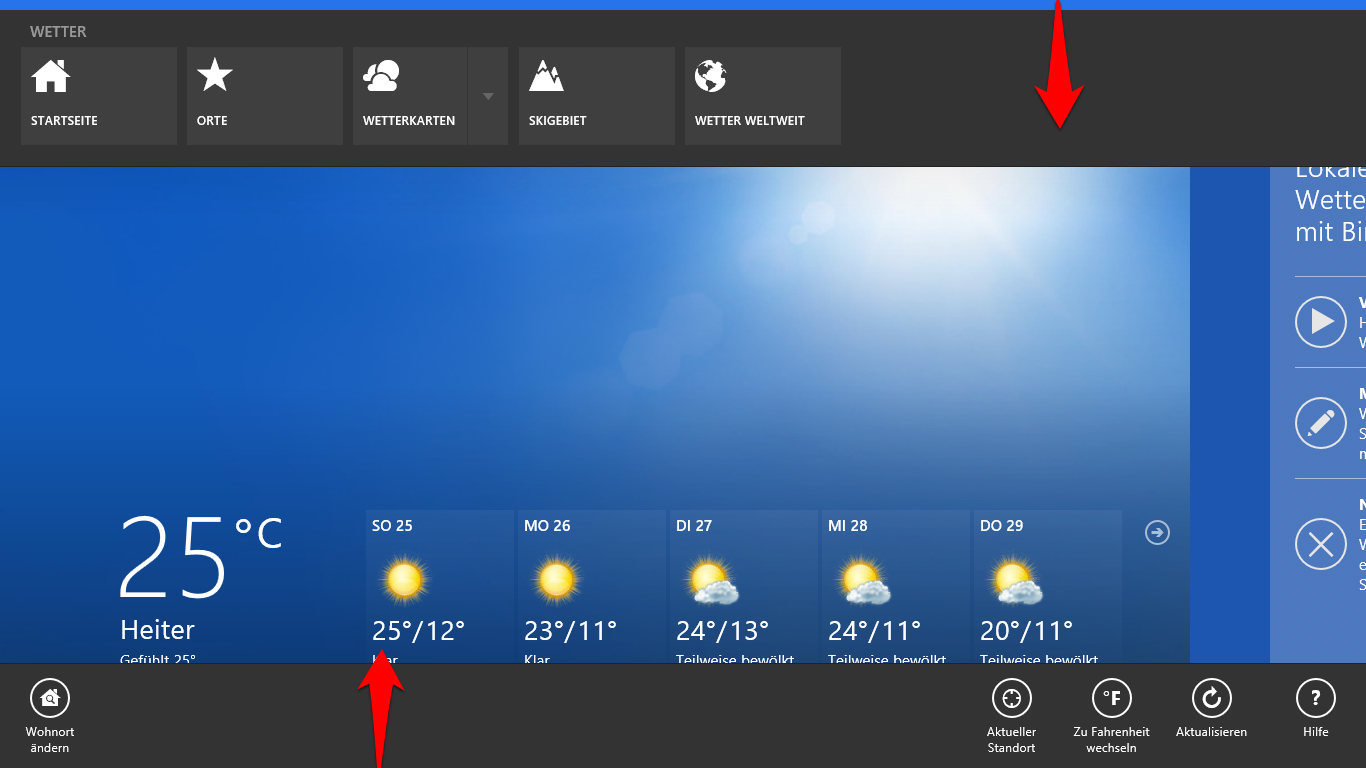
\includegraphics[width=0.6\textwidth]{Bilder/Screenshots/windows8/app_leisten.png} 
	\caption{Geste zum Öffnen der unteren und oberen Menüleisten.}
	\label{fig:menubar}
\end{figure}  

\subsection{Windows 8 als hybrides System}
\label{subsec:hybrides system}
% touch, vorteile, nachteile
Windows 8 kann sowohl auf herkömmlichen Desktop Computern, Notebooks und auf Tablet-Computern eingesetzt werden. 
\subsection{Windows RT}
\label{subsec:winRT}
\subsection{Das Ökosystem}
\label{subsec:ökosystem}
\subsubsection{Microsoft Store}
\label{subsubsec:store}
\subsubsection{Windows Phone}
\label{subsubsec:windowsphone}

\newpage
\section{Bildsprache}

\newpage
\section{Konzeption der App}
\label{sec:konzeption}
In dieser Sektion wird zunächst ein Blick auf die ZEIT ONLINE Webseite und auf bereits vorhandene ZEIT ONLINE Apps geworfen. Anschließend es darum, die Konzeption für eine Windows 8 Nachrichten App darzustellen und zu erläutern. Dabei gilt es darzulegen, warum und mit welchem Hintergrund Entscheidungen zu Gunsten der einen oder der anderen Möglichkeit ausfallen. Dazu müssen zunächst die Ziele der App ausgeführt werden. Anschließend muss sich entschieden werden mit welcher Technologie bzw. Programmiersprache gearbeitet werden soll. Zuletzt wird noch ein detaillierterer Blick auf das Herzstück der App geworfen. Das Navigationskonzept. Hierbei ist eine der wichtigsten Fragen: \glqq Wie kann ich auch bei ggf. großen Datenmengen eine übersichtliche, intuitive Struktur schaffen die sich in das Gesamtkonzept von Windows 8 eingliedert?\grqq  

\subsection{ZEIT ONLINE}
\label{subsec:zeitonline}

\subsubsection{Die Webseiten}
\label{subsubsec:webseiten}

\subsubsection{Die iPad App}
\label{subsubsec:ipadapp}

\subsubsection{Die Webapp}
\label{subsubsec:webapp}




\subsection{Ziel der App}
\label{subsec:zielderapp}
Das Ziel der zu erstellenden App ist, den Inhalt der ZEIT ONLINE Website auf ansprechende Art und Weise in einer Windows 8 Applikation darzustellen. Das Layout und die Darstellung der Inhalte soll sich an das sogenannte \glqq Look and Feel\grqq\ von Windows 8 anpassen und sich daran orientieren. Der Fokus bei den Inhalten liegt auf den Artikeln selbst und den jeweiligen Aufmacher bzw. Teaser Bildern. Das heißt andere Inhalte wie z.B. Bildergalerien, Infografiken, Blogartikel oder Quizze werden von der App nicht erfasst und nicht dargestellt. Hintergrund ist, die App möglichst einfach zu halten da es in der Fragestellung um die Relation zwischen den Aufmacherbildern und dem dahinter liegenden Artikeltext geht. Die App erhebt in dieser Hinsicht keinen Anspruch darauf, die gesamten redaktionellen Inhalte von \mbox{ZEIT ONLINE} darzustellen, sondern versteht sich eher als explorative Applikation im Sinne der Fragestellung.\\
Der User soll die Möglichkeit haben die standardmäßig vorhandenen Artikeltitel auszublenden um so, wenn gewünscht, einen rein visuellen Eindruck der Artikelbilder zu bekommen. Hierzu soll einen Schalter in der Menüleiste am unteren Bildrand geben. Wenn der User sich im Artikel befindet soll er die Möglichkeit haben die Schriftgröße in gewissen Maß selbst zu bestimmen, da die App eventuell auf Monitoren mit verschieden großen Auflösungen ausgeführt werden wird oder die Sehkraft des Users nicht mehr ausreicht um eine normal große Schrift zu erkennen und zu lesen. So wird in den Artikeln ein gewisses Maß an Barrierefreiheit gewährleistet.\\
Das übergeordnete Ziel der App ist es, eine rudimentäre Nachrichten Applikation für Windows 8 zu erstellen. Gleichzeitig soll eine Umgebung geschaffen werden, die es erlaubt Untersuchungen anzustellen, in wie weit es möglich ist allein durch das Betrachten der Aufmacherbilder auf den Inhalt der jeweiligen Artikel zu schließen (siehe Sektion \ref{subsubsec:nurbildermodus} auf Seite \pageref{subsubsec:nurbildermodus}). Außerdem soll die App dazu dienen, zu erforschen, wie eine Nachrichten Applikation in der Modern UI Oberfläche von Windows 8 erstellt wird und welche design- als auch funktionstechnischen Vorgaben von Microsofts vorhanden sind. Sprich, wie eine App mit Nachrichteninhalten nach Microsofts Sichtweise auszusehen hat. 


\subsection{Navigationskonzept}
\label{subsec:navikonzept}
Damit der User ein für ihn angenehmes und flüssiges Nutzungserlebnis hat, ist es notwendig sich über das Navigationskonzept Gedanken zu machen, gerade wenn es sich um eine App handelt, in der es viele verschiedene Inhaltsbereiche gibt. Der User soll sich möglichst intuitiv durch die Inhalte bewegen können. Außerdem muss dem User auf der Einstiegsebene der ein guter Überblick über die vorhandenen Inhalte gegeben werden, damit er von dort aus zielgerichtet weiter navigieren kann, ohne lange suchen zu müssen. Microsoft nennt in seinen Richtlinien für Windows Store Apps (Modern UI Apps) grundsätzlich zwei Möglichkeiten wie die Navigation umgesetzt werden kann.

\subsubsection{Flaches System}
\label{subsubsec:flachessystem}
Das flache Navigationssystem wird in vielen Windows Store Apps verwendet, häufig in Spielen, Browsern oder in Apps zum Erstellen von Dokumenten. Es zeichnet sich dadurch aus, dass sich die Inhalte auf der gleichen hierachischen Ebene befinden. Dieses System eignet sich wenn ein schneller Wechsel zwischen wenigen Seiten oder Registerkarten möglich sein soll \citep{MicrosoftNavidesign2013}.

\begin{figure}[h]	
	\centering
	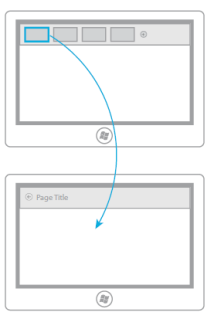
\includegraphics[scale=1]{Bilder/Abbildungen/ms_navigation_flach.png} 
	\caption{Flaches Navigationssystem \protect\citep{MicrosoftNavidesign2013}.}
	\label{fig:naviflach}
\end{figure}

Abbildung \ref{fig:naviflach} zeigt wie das flache Navigationssystem funktioniert. Am oberen Rand befindet sich eine, nicht immer sichtbare Navigationsleiste mit den verschiedenen Registerkarten oder Seiten. Die Leiste wird angezeigt, wenn der User vom unteren oder oberen Bildrand streift (siehe Sektion \ref{subsec:bedienkonzept}). Wenn der User die Seite wechseln möchte geschieht dies  direkt über die Navigationsleiste, d.h. es gibt meist keinen permananten Zurück-Button. Ein flaches Navigationssystem eignet sich nicht unbedingt für eine Nachrichten App wie die, die in dieser Arbeit konzipiert und umgesetzt ist, weil es zu viele Bereiche (Ressorts) gibt, welche sich zudem sehr ähneln. Hier ist es angebracht ein hierarchisches Navigationssystem zu verwenden.    



\subsubsection{Hierarchisches System}
\label{subsubsec:hierachischessystem}
Die meisten Windows Store-App benutzen ein hierarchisches Navigationssystem. Microsoft nennt es Hubnavigationsmuster. Es eignet sich um große Inhaltssammlungen zu ordnen und sie für User benutzerfreundlich auf zu bereiten. Der Schlüssel dazu ist die Unterteilung des Inhalts in verschiedene Detailebenen \citep{MicrosoftNavidesign2013}.

\begin{figure}[h]	
	\centering
	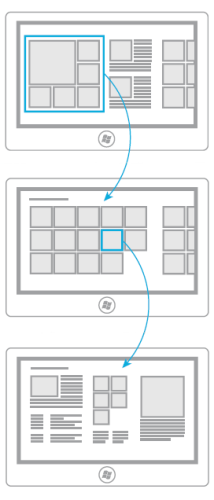
\includegraphics[scale=1]{Bilder/Abbildungen/ms_navigation_hierarchie} 
	\caption{Hierarchisches Navigationssystem \protect\citep{MicrosoftNavidesign2013}.}
	\label{fig:navihierarchisch}
\end{figure}

Das Schema eines hierarchischen Systems ist in Abbildung \ref{fig:navihierarchisch} dargestellt. Der Einstiegspunkt in die App ist die sogenannte \glqq Hubseite\grqq\, hier ganz oben in der Abbildung zu sehen. Auf der Hubebene werden aus den vielen großen Bereichen der App jeweils ein kleiner Teil gesammelt und dargestellt, sodass sich der User vorstellen kann was ihn im jeweiligen Bereich erwartet. Die Anordnung, in welcher der Auszug der Inhalte dargestellt ist muss nicht für jeden Bereich gleich sein. Es kann das Nutzungserlebnis sogar verbessern und vielfältiger machen wenn unterschiedliche Darstellungen (z.B. in Höhe, Breite oder Anzahl der Objekte) für die Bereiche genutzt werden. Die Hubansicht wird horizontal gescrollt, d.h. weiterer Inhalt befindet sich hinter dem rechten Rand und kann entweder durch das Scrollrad der Maus oder auf einem Tablet, durch das swipen nach links in das Sichtfeld des Users gebracht werden.\\
Die mittlere Darstellung in Abbildung \ref{fig:navihierarchisch} zeigt die zweite Detailstufe des hierarchischen Systems. Hier werden alle Elemente eines Bereichs dargestellt. In diesem Fall werden hier alle Artikel aus einem Ressort aufgelistet.\\
Im unteren Bereich der Abbildung ist schließlich die letzte Detailstufe zu sehen. Es handelt sich hierbei um den eigentlichen Inhalt (z.B. einen Artikel). Es ist ebenfalls möglich von der Hubansicht direkt in die Detailansicht eines Elements zu wechseln.  

\begin{figure}[h]	
	\centering
	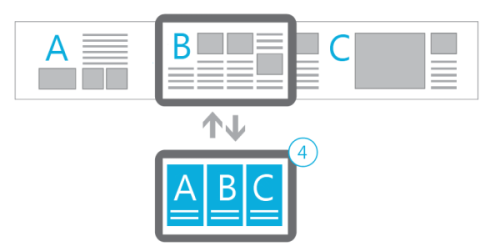
\includegraphics[scale=1]{Bilder/Abbildungen/ms_navigation_hierarchie_semantic_zoom} 
	\caption{Schema des \glqq Semantic Zoom\grqq\ \protect\citep{MicrosoftNavidesign2013}.}
	\label{fig:semanticzoomkonzept}
\end{figure}

Befinden sich in der Hubansicht, trotz der Zusammenfassung der Bereiche noch zu viele Bereiche und es dauert zu lange bis zum Ende zu scrollen, kann man noch eine weitere Ebene \glqq davor\grqq\ legen. Das Konzept nennt Microsoft \glqq Semantic Zoom\grqq\ und ist in Abbildung \ref{fig:semanticzoomkonzept} schematisch dargestellt. Oben in der Abbildung ist die Hubansicht dargestellt, unten die zusätzliche semantic Zoom Ebene. In der Praxis kann der User auf diese Weise die Inhalte noch weiter vereinfachen und zusammenfassen lassen. Im Fall dieser App soll es einen semantischen Zoom geben, um ein flüssigeres und schnelleres Navigieren z.B. ganz zum Ende der Hubansicht zu ermöglichen, da es über zehn verschiedene Ressorts geben wird. Diese Ansicht soll nur die Namen der verschiedenen Ressorts, sowie ein zufälliges Bild aus dem jeweiligen Ressort zeigen. Um am Desktop-PC (mit Maus) diese Ansicht aufzurufen, muss der User auf ein kleines Minuszeichen am unteren rechten Rand klicken. Am Tablet wird der semantische Zoom mit der \glqq Pinch to Zoom (out)\footnote{Pinch to Zoom erklären}\grqq\  Geste aufgerufen. Klickt der User auf ein Element in dieser zusätzlichen Navigationsebene, wird er direkt zum jeweiligen Ausschnitt in die Hubansicht navigiert. Die semantic Zoom Ansicht kann von überall aus der Hubansicht aufgerufen werden.  


\subsection{Nativ vs. Web}
\label{subsec:nativ_vs_web}
Vor dem Entwickeln einer Windows 8 App muss sich entschieden werden mit welcher Technologie bzw. mit welcher Programmiersprache entwickelt werden soll. Die Rede ist hier von einer App die in der Modern UI Oberfläche von Windows 8 läuft und für diese konzipiert ist. Das heißt es handelt sich nicht um eine klassische .NET oder WIN32 Anwendung für Windows. Um eine Modern UI App zu entwickeln, müssen zwei Dinge zwingend vorhanden sein. Zum einen Windows 8 selbst und zum anderen wird die neueste Version von Visual Studio, Visual Studio 11\footnote{Visual Studio 2011 war die aktuellste Version beim Erstellen dieser Arbeit.}, benötigt. Visual Studio steht in der Express Version für Windows 8 kostenlos zur Verfügung. Des weiteren muss sich zwischen der nativen Umsetzung und der Implementierung mit Webtechnologien entschieden werden. Es soll zunächst erläutert werden was die beiden Begriffe bedeuten und in welcher Weise und welchem Zusammenhang sie bei der Entwicklung einer Windows 8 Modern UI App üblicherweise gebraucht werden.

\subsubsection{Native App}
\label{subsubsec:nativ}
Der heutige Begriff \glqq native App\grqq\ unterscheidet sich in einigen Punkten von der früheren oder ursprünglichen Verwendung des Begriffs. Früher sprach man von einer nativen App wenn direkt auf die Ressourcen der  Maschine zugegriffen wurde, wie z.B. Maschinencode der direkt von der CPU ausgeführt wird. Heute wird eine App oftmals schon als nativ deklariert, wenn es sich nicht um eine Webapp handelt. Eine sinnige Definition liegt irgendwo zwischen diesen beiden Varianten. Eine App ist dann nativ, wenn sie Geräte- , Betriebssystem- oder Laufzeitumgebungsabhängig ist. Das heisst, sie ist für ein spezielles Gerät entwickelt und kann nur auf diesem ausgeführt werden. Sie kann dabei alle Geräte- oder Betriebssystemspezifischen Funktionen nutzen, es ist jedoch egal wie nah an der Hardware tatsächlich programmiert wurde \citep{OBrian2013}.\\
In Visual Studio können native Windows 8  Apps u.a. mit den Programmiersprachen C++, C\# oder Visual Basic erstellt werden. Für das Design bzw. das Aussehen der App wird die Markupsprache - \ac{xaml} - verwendet. Es gibt zwei Möglichkeiten wie das \ac{xaml} erstellt werden kann. Es kann entweder von Hand geschrieben werden oder man lässt es sich automatisch generieren. Zum automatischen Generieren lassen sich per Drag \& Drop Elemente wie z.B. Buttons und andere Schaltflächen aus einer Werkzeugpalette direkt auf die \glqq App-Leinwand\grqq\ ziehen, sowie verschieben oder nach Belieben anordnen.
%Listing XAML oder Screenshot 

\subsubsection{Windows 8 App mit Webtechnologien}
\label{subsubsec:webwin8}

  


\subsection{Menü und Features}
\label{subsec:menuandproperties}
Da die App einen explorativen Charakter hat wird sich bei den Funktionen und Features auf das nötigste beschränkt. Es soll eine untere App-Leiste geben, in welcher, je nach dem in welcher Ansicht sich der User gerade befindet verschiedene Optionen angezeigt werden. Diese Leiste ist nicht dauerhaft zu sehen und kann, wenn man mit der Maus arbeitet durch einen Rechtsklick aufgerufen werden. Auf einem Tablet geschieht dies durch swipen vom oberen oder unteren Bildschirmrand.\\
In der Startansicht, sowie in der Ressortübersicht soll es am unteren Bildrand die Möglichkeit geben, die Titel aller Elemente aus- bzw. auch wieder einzublenden um so dem User ein rein visuelles Erleben der Artikelbilder zu ermöglichen. In der Artikelansicht soll der User die Möglichkeit haben, die Schriftgröße des Artikels zu vergrößern, zu verkleinern, sowie die Schriftgröße wieder auf ihren Startwert zu setzen. 

\newpage
\section{Umsetzung der App}
\label{sec:umsetzungderapp}

\subsection[Rastervorlage] {Rastervorlage\footnote{Die Namen der verwendeten Dateien in der Rastervorlage wurden mittlerweile von Microsoft geändert.}}
\label{subsec:rastervorlage}
Beim Erstellen einer Windows 8 Modern UI App mit \ac{html} und Javascript bietet Microsoft von Haus aus verschiedene Vorlagen für Visual Studio, welche schon einige Grundfunktionen besitzen und sich so als guter Startpunkt für eine weiterführende App eignen. Die Vorlage die für diese App verwendet wird ist die Raster-App (engl. Grid Application) Vorlage. Sie bietet die Grundarchitektur für ein hierarchisches Navigationssystem wie es in Sektion \ref{subsubsec:hierachischessystem} auf Seite \pageref{subsubsec:hierachischessystem} beschrieben ist.\\
Es wird von Microsoft empfohlen, dass Windows-Store Apps, welche mit \ac{html} und Javascript erstellt werden das single-page Navigationmodell verwenden. Das bedeutet, die Navigation erfolgt nicht über Hyperlinks, sondern die verschiedenen Inhalte werden direkt in die Seite nachgeladen (ähnlich wie ein iframe). Auf diese Weise gibt keine Sichtbare Unterbrechung beim Navigieren (der Bildschirm wird nicht kurz weiß beim Navigieren). Außerdem erzielt man auf diese Weise eine bessere Performance und die App fühlt sich mehr \glqq app-like\grqq\ an. Die Rastervorlage verwendet das single-page Navigationsmodell \citep{MicrosoftSinglePage2013}. Abbildung \ref{fig:projektmappe} zeigt die Dateistruktur des Projektes. Anschließend wird kurz erläutert wofür die einzelnen Dateien da sind.

\begin{figure}[h]
	\centering
	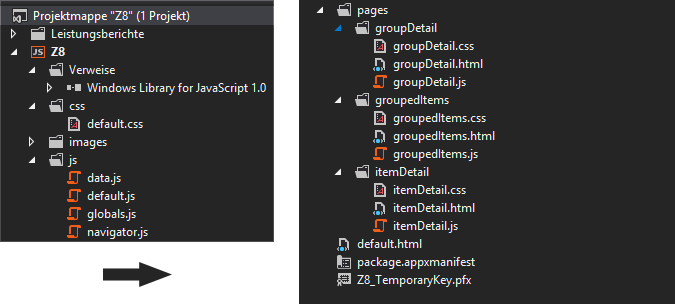
\includegraphics[width=\textwidth]{Bilder/Screenshots/app/projektmappe.png} 
	\caption{Die Projektstruktur in Visual Studio.}
	\label{fig:projektmappe}
\end{figure}

\subsubsection{HTML Dateien}
\label{subsubsec:htmldateien} 
Folgende \ac{html} Dateien sind bereits in der Raster-App Vorlage enthalten:
\begin{description}
	\item[default.html], wird als erstes geladen und enthält das \ac{html} für den Inhalthost (dies ist die Seite in welche die anderen Inhalte im Zuge der single-page Navigation herein geladen werden).
	\item[groupedItems.html], ist der Einstiegspunkt in die App (die Hubansicht).
	\item[groupDetail.html], zeigt alle Elemente eines Bereichs.
	\item[itemDetail.html], Einzelansicht eines Elements.
\end{description}

\subsubsection{Javascript Dateien}
\label{subsubsec:javascriptdateien} 
Folgende Javascript Dateien sind bereits in der Raster-App Vorlage enthalten:
\begin{description}
	\item[default.js], legt fest wie sich die App beim Start verhält.
	\item[groupedItems.js | groupDetail.js | itemDetail.js], sind die Javascript Dateien, welche das Verhalten für die gleichnamigen \ac{html} Dateien festlegen.
	\item[navigator.js], implementiert das hierarchische Navigationssystem, sowie das single-page Navigationmodell.
	\item[data.js], stellt die benötigten Daten für den Rest der App bereit.
\end{description}

\subsubsection{CSS Dateien}
\label{subsubsec:cssdateien} 
\begin{description}
	\item[default.css], enthält Styles für Inhaltshostseite, sowie für die gesamte App.
	\item[groupedItems.css | groupDetail.css | itemDetail.css], 
\end{description}
Diese Vorlage wird nachfolgend angepasst und verändert, sodass sie die konzeptionierten Anforderungen erfüllt.

\subsection{Datenanbindung}
\label{subsec:datenanbindung}

\subsubsection{ZEIT ONLINE Datenbestand}
\label{subsubsec:zondatenbestand}
Es soll zunächst geklärt werden wie sich der Inhalt der ZEIT ONLINE Website darstellt und wie er generiert wird. Die redaktionellen Inhalte werden fast ausschließlich über ein hauseigenes \ac{cms} erstellt und gepflegt. Das \ac{cms} generiert aus den Inhalten eine \ac{xml}-Struktur. Aus dem \ac{xml} wiederum wird anschließend mit Hilfe von \ac{xslt} in einer zweistufigen Transformation das fertige \ac{html} erstellt. Dies ist ein grober Überblick wie sich die Webseite von ZEIT ONLINE zusammensetzt.\\
Für die Windows 8 App wird direkt das \ac{xml} verwendet, welches vom \ac{cms} generiert wird. Für die App werden zwei verschiedene Seitentypen der Webseite benötigt um die gewünschten Informationen darzustellen. Zum einen die verschiedenen \glqq Centerpages\grqq\ und zum anderen die Artikelansicht. Centerpages sind die Hauptseiten der jeweiligen Ressorts (z.B. die Hauptseite des Politikressorts), sowie die Startseite mit den wichtigsten und aktuellsten Meldungen. Auf den Centerpages befinden sich die Teaserelemente für die verschiedenen Artikel. Die Teaserelemente bestehen meist aus einem Bild und einem kurzen, prägnanten Text, welcher kurz erläutert worum es in dem dahinter liegenden Artikel geht.\\

\begin{minipage}{\linewidth}
\begin{lstlisting}[language= XML,caption=Das XML eines Teaserelements, label={lst:knopfxml}]
<block href="http://xml.zeit.de/digital/internet/2013-08/fablab-open-hardware" year="2013" issue="34" ressort="Digital" author="Tilman Baumgärtel" contenttype="article" publication-date="" expires="" date-last-modified="2013-08-14T12:58:40+00:00" date-first-released="2013-08-14T09:57:43.627551+00:00" date-last-published="2013-08-14T12:59:39.691370+00:00" last-semantic-change="2013-08-14T09:56:40.185797+00:00">
	<supertitle>Open Hardware</supertitle>
	<title>Fab Labs, die Maschinen-Bibliotheken</title>
	<text>
		3-D-Drucker, CNC-Fräsen oder Lasercutter - mit solchen Maschinen sollen Bastler in Fab Labs experimentieren. Immer mehr solcher Werkstätten entstehen nun in aller Welt.
	</text>
	<description>
		3-D-Drucker, CNC-Fräsen oder Lasercutter - mit solchen Maschinen sollen Bastler in Fab Labs experimentieren. Immer mehr solcher Werkstätten entstehen nun in aller Welt.
	</description>
	<byline/>
	<image alt="MakerBot Replicator 2" align="left" title="MakerBot Replicator 2" base-id="http://xml.zeit.de/digital/internet/2013-08/makerbot-cebit-hannover/" type="jpg" publication-date="" expires="">
		<bu>
			Ein MakerBot Replicator 2 auf der diesjährigen Cebit in Hannover
		</bu>
		<copyright>© REUTERS/Fabrizio Bensch</copyright>
	</image>
</block>
\end{lstlisting}


\end{minipage}

Das \ac{xml} von einem Teaserelement ist in Listing \ref{lst:knopfxml} dargestellt. Es werden jedoch nicht alle Informationen aus dem \ac{xml} verwendet. Die verwendeten Informationen sind das \glqq date-first-released\grqq\ (Zeile 1), der \glqq title\grqq\ (Zeile 3), sowie die \glqq description\grqq\ (Zeile 7) und das \glqq image\grqq\ (Zeile 11). Das \ac{xml} für die Artikelansicht ist ähnlich aufgebaut, nur ist hier zusätzlich noch der Artikeltext (Inhalt) in Form von Paragraphen-Tags (<p>) enthalten. Dies ist ein konkreter Einblick wie die rohen Daten aussehen, welche für die App verwendet werden. Wie die Daten im Detail verarbeitet werden wird in der nächsten Sektion erläutert.

\subsubsection{Daten verfügbar machen}
\label{subsubsec:datenverfügbarmachen}
Die Daten, die in der App dargestellt werden sollen, werden grundsätzlich in zwei Schritten geladen. Wenn die App startet werden zunächst alle benötigten Daten außer den eigentlichen Artikeln geladen. Der Artikelinhalt wird erst geladen, wenn der User ihn lesen will. Dies spart Zeit beim starten der App und der User hat somit ein flüssigeres App-Erlebnis. Der erste Schritt beim Daten Einlesen und Verarbeiten geschieht in der \glqq data.js\grqq\ Datei. Es werden alle Teaser Elemente aller Ressorts letztendlich in einer \glqq WinJS.Binding.List()\grqq\ gespeichert und für den weiteren Gebrauch verfügbar gemacht. Die \ac{winjs} ist eine Javascript Bibliothek für Windows-Store Apps, die mit Javascript erstellt werden. Sie enthält nützliche Funktionen z.B. für UI Steuerelemente oder sie hilft beim \ac{xhr}. Die Binding.List ist ebenfalls ein Teil dieser Bibliothek. Sie stellt Logik für die Datengruppierung bereit, genau in der Art und Weise wie es für diese App sinnvoll ist. Falls mit dynamischen Daten gearbeitet wird stellt sie z.B. Funktionen für die automatische Aktualisierung der Daten bereit.In Listing \ref{lst:bindinglst} ist die Initialisierung einer WinJS.Binding.List dargestellt.

\begin{minipage}{\linewidth}
\begin{lstlisting}[language= Javascript,caption=Initialisierung der Binding-List., label={lst:bindinglst}]
var teaserElements = new WinJS.Binding.List();
\end{lstlisting}
\end{minipage}

Die Grundinformationen zu den einzelnen Ressorts, wie der Name und die URL, werden zunächst als normales Javascript Array festgelegt. Einen Beispieleintrag aus dem Array zeigt Listing \ref{lst:ressortsarray}.

\begin{minipage}{\linewidth}
\begin{lstlisting}[language= Javascript,caption=Auszug aus dem Ressorts Array., label={lst:ressortsarray}]
ressorts = [
	{
	    key: "ressort01", url: 'http://xml.zeit.de/index',
	    title: 'Top Stories', subtitle: 'subtitle', updated: 'tbd',
	    backgroundImage: 'tbd', articleLink: "tdb",
	    acquireSyndication: acquireSyndication, dataPromise: null
    }
]
\end{lstlisting}
\end{minipage}

Anschließend wird eine weitere Funktion von \ac{winjs} verwendet, die WinJS.Promises. Mit Promises kann mit asynchronen Prozessen und Datenquellen umgegangen werden. Hier werden für alle Ressorts \ac{xhr}s gestartet, an die im Ressorts-Array angegebene URLs. Alle \ac{xhr}s werden ebenfalls in einem Array gespeichert und erst wenn alle Promises vorhanden sind (alle URL waren erreichbar), wird die Datenverarbeitung fortgesetzt. \\
Mit den vorhandenen und validen \ac{xhr} Responses können anschließend alle Teaserelemente in einer Schleife durchlaufen, das \ac{xml} geparst und so die nötigen Informationen für die App verfügbar gemacht werden. Listing \ref{lst:xmlparsing} zeigt wie der Titel (Zeile 10), der Teasertext (Zeile 13) und der Bildpfad (Zeilen 15-22) aus dem \ac{xml} gewonnen werden. Am Ende der Funktion werden die Daten in die in Listing \ref{lst:bindinglst} erstellte WinJS.Binding.List geschrieben (Zeilen 24-28). Die dargestellte Funktion ist nicht vollständig und wurde aus Übersichts- und Relevanzgesichtspunkten verkürzt dargestellt.

\begin{minipage}{\linewidth}
\begin{lstlisting}[language= Javascript,caption=Parsen und Speichern der Daten., label={lst:xmlparsing}]
function getItemsFromXml(ressortXML, teaserElements, ressort) {
    var teasers = ressortXML.querySelectorAll("region[area='lead'] container > block:first-child");
    // Process each ressort teaser.
    for (var teaserIndex = 0; teaserIndex < teasers.length; teaserIndex++) {
        var teaser = teasers[teaserIndex];

       //only articles with an image are alllowed
        if (teaser.getAttribute("contenttype") == "article" && teaser.querySelector("image") !== null) {
            // Get the title
            var teaserTitle = teaser.querySelector("title").textContent;
        
            // Process the content so that it displays nicely.
            var staticContent = toStaticHTML(teaser.querySelector("description").textContent);

            //Get and build the image path
            var teaserImageEl = teaser.querySelector("image");
            var imageBasePath = teaserImageEl.getAttribute("base-id");
            var splitImagePath = imageBasePath.split('/');
            var imageNameSmall = splitImagePath[splitImagePath.length - 2] + "-220x124.jpg";
            var imageNameBig = splitImagePath[splitImagePath.length - 2] + "-540x304.jpg";
            var imagePathSmall = imageBasePath + imageNameSmall;
            var imagePathBig = imageBasePath + imageNameBig;
            
            // Store the teaser element info we care about in the array.
            teaserElements.push({
                group: ressort, key: ressort.title, title: teaserTitle,
                backgroundImage: imagePathBig, teaserText: staticContent
            });
        }
    }
}
\end{lstlisting}   
\end{minipage}

Sobald die Daten in der WinJS.Binding.List gespeichert sind können sie vom Rest der App weiterverwendet und grafisch aufbereitet werden. Es wurden bisher noch keine Artikelinhalte geladen, dies geschieht erst wenn der User auf einen Artikel klickt.

\subsection{Darstellung der Daten}
\label{subsec:darstellungderdaten}

\subsubsection{Die Hubansicht}
\label{subsubsec:hubansicht}
Wenn die App startet befindet sich der User in der Hubansicht. Hier werden ihm für alle Hauptressorts die ersten sechs Artikel angezeigt, in der Reihenfolge wie sie auch auf der Webseite zu finden sind (siehe Abbildung \ref{fig:hubressortübersicht}).\\
Zu der Hubansicht gehören eine \ac{html} Datei, in welcher das Markup festgelegt ist, eine CSS Datei, die das Layout der Seite bestimmt und eine Javascript Datei, in welcher das Verhalten (die Logik) der Hubseite programmiert wird. 

\begin{figure}[h]
	\centering
	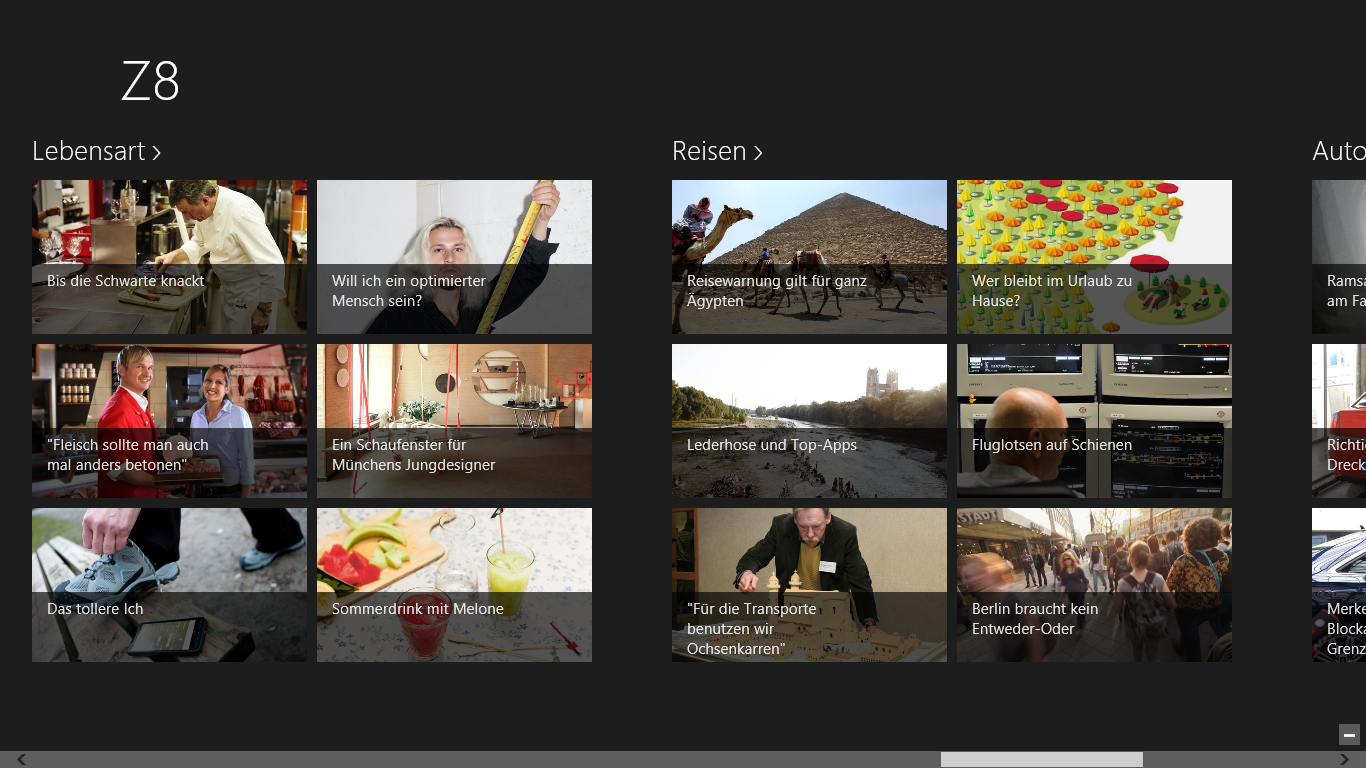
\includegraphics[width=\textwidth]{Bilder/Screenshots/app/reise_aegypten_2gmit.png} 
	\caption{Die Hubansicht.}
	\label{fig:hubressortübersicht}
\end{figure}

Um die Daten aus der \textit{WinJS.Binding.List} auf der Hubseite anzeigen zu können, sind einige Schritte notwendig. Zunächst soll der Aufbau der \ac{html} Datei erläutert werden. Listing \ref{lst:hubmarkup} zeigt einen Ausschnitt aus der \textit{groupedItems.html} Datei. Im oberen Teil befindet sich ein Template mit der Klasse \textit{itemtemplate}, welches auf jedes einzelne Element der Hubansicht angewandt wird. Das besondere an diesem Template ist, dass es ein \textit{data-win-control} Attribut mit dem Wert \glqq WinJS.Binding.Template\grqq\ besitzt. Dies bedeutet, es akzeptiert Daten aus einer \textit{WinJS.Binding.List}, wie sie in der Rohdatenverarbeitung genutzt wurde. Im unteren Teil ab Zeile 10 ist der Container für den eigentlichen Inhalt. Dieses Objekt besitzt ein \textit{data-win-control} Attribut mit dem Wert \glqq WinJS.ListView\grqq\ . Eine \textit{WinJS.LisView} stellt Elemente in anpassbaren Listen oder Rastern dar. 

\begin{minipage}{\linewidth}
\begin{lstlisting}[language= XML,caption=Die wichtigsten Markupelemente der Hubansicht., label={lst:hubmarkup}]
<div class="itemtemplate" data-win-control="WinJS.Binding.Template">
    <div class="item">
        <img class="item-image" src="#" data-win-bind="src: backgroundImage; alt: title" />
        <div class="item-overlay">
            <h4 class="item-title" data-win-bind="textContent: title"></h4>
        </div>
    </div>
</div>

<section aria-label="Main content" role="main">
    <div class="groupeditemslist win-selectionstylefilled" aria-label="List of groups" data-win-control="WinJS.UI.ListView" data-win-options="{selectionMode: 'none'}"></div>
</section>
\end{lstlisting}   
\end{minipage}

Der Rest passiert in der \textit{groupedItems.js} Datei. Die \textit{groupedItems.js} besitzt eine \textit{ready()} Methode. Diese wird jedesmal aufgerufen, wenn der User zur Hubansicht wechselt oder die Hubansicht wiederhergestellt wird. Um die Daten in die \textit{WinJs.ListView} zu bekommen wird als erstes die \textit{WinJS.ListView} in einer Variable gespeichert und anschließend das gewünschte Template bei der ListView registriert (siehe Listing \ref{lst:getitemtemplate}). 

\begin{minipage}{\linewidth}
\begin{lstlisting}[language= Javascript,caption=Template bei der Listview registrieren., label={lst:getitemtemplate}]
var listView = element.querySelector(".groupeditemslist").winControl;
listView.itemTemplate = element.querySelector(".itemtemplate");
\end{lstlisting}   
\end{minipage}

Anschließend wird die \textit{initializeLayout} Funktion aufgerufen. Hier wird am Anfang eine entscheidende Operation ausgeführt. In der \textit{WinJS.Binding.List} sind bisher alle Teaserelemente aus allen Ressorts enthalten, für die Hubansicht sind aber nur sechs Elemente pro Ressort gewünscht. Deswegen wird eine Funktion \textit{getClippedList()} in der \textit{data.js} Datei aufgerufen, welche die ersten sechs Elemente jedes Ressorts zurück liefert. Damit die Elemente wie gewünscht angezeigt werden können, muss noch die \textit{dataSource} der \textit{WinJS.ListView} gesetzt werden, ebenso wie das Raster-Layout (siehe Listing \ref{lst:setdatasource}). Nach diesem Schritt werden die ersten sechs Elemente jedes Ressorts wie in Abbildung \ref{fig:hubressortübersicht} angezeigt.

\begin{minipage}{\linewidth}
\begin{lstlisting}[language= Javascript,caption=Setzen der Datenquelle und des Layouts., label={lst:setdatasource}]
listView.itemDataSource = groupedItemsHub.dataSource;
listView.layout = new ui.GridLayout({ groupHeaderPosition: "top" });
\end{lstlisting}   
\end{minipage}

\subsubsection{Die Ressortansicht}
\label{subsubsec:ressortansicht}
Die Ressortansicht, die zweite Detailstufe zeigt alle Elemente eines Ressorts (siehe Abbildung \ref{fig:einzelressortübersicht}). Der User gelangt hierhin wenn er in der Hubansicht auf den Ressortnamen im Headerbereich klickt. 

\begin{figure}[h]
	\centering
	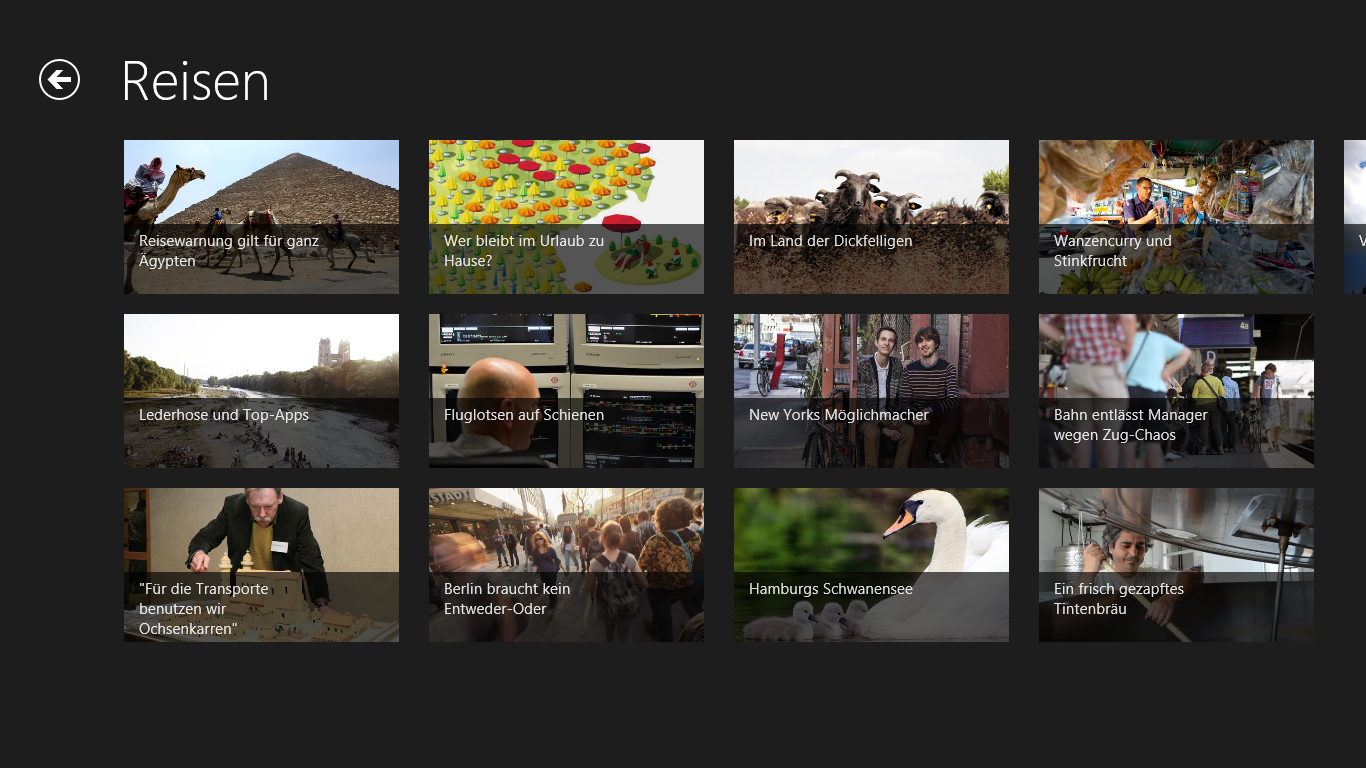
\includegraphics[width=\textwidth]{Bilder/Screenshots/app/reise_aegypten_3gdmit.png} 
	\caption{Die Einzelressortübersicht (hier das Reisen Ressort).}
	\label{fig:einzelressortübersicht}
\end{figure}

Die Programmlogik funktioniert analog zur Hubansicht. Es werden die gleichen Mechanismen zur Darstellung des Raster-Musters benutzt. Auch die zu dieser Ansicht gehörende \ac{html} und Javascript Dateien ähneln denen von der Hubansicht sehr. Ein wesentlicher Unterschied ist, dass im Gegensatz zu Hubansicht nicht die Funktion \textit{getClippedList()}, sondern stattdessen die Funktion \textit{getItemsFromGroup()} aufgerufen wird. Sie gibt alle Elemente der übergebenen Gruppe zurück. Diese können nun mit einem \textit{itemTemplate} und einer \textit{WinJS.ListView} dargestellt werden. 

\subsubsection{Die Artikelansicht}
\label{subsubsec:artikelansicht}
Die Artikelansicht ist die letzte Detailstufe. Sie zeigt den eigentlichen Artikelinhalt (siehe Abbildung \ref{fig:artikelansicht}). Dargestellt wird das Ressort, der Titel, der Teasertext, das Aufmacherbild in groß, die Bildunterschrift, das Copyright für das Bild, der Artikeltext, die Quelle des Artikels (z.B. ZEIT ONLINE oder dpa), der Autor sowie das Erstellungsdatum. Die Artikeldarstellung funktioniert etwas anders als die Hub- und der Ressortdarstellung. Es wird kein Template verwendet, stattdessen wird das \ac{html} mit Hilfe von Javascript befüllt. In der \textit{ready()} Funktion der \textit{itemDetail.js} Datei werden zunächst die bereits vorhandenen Information in das \ac{html} eingefügt.

\begin{figure}[h]
	\centering
	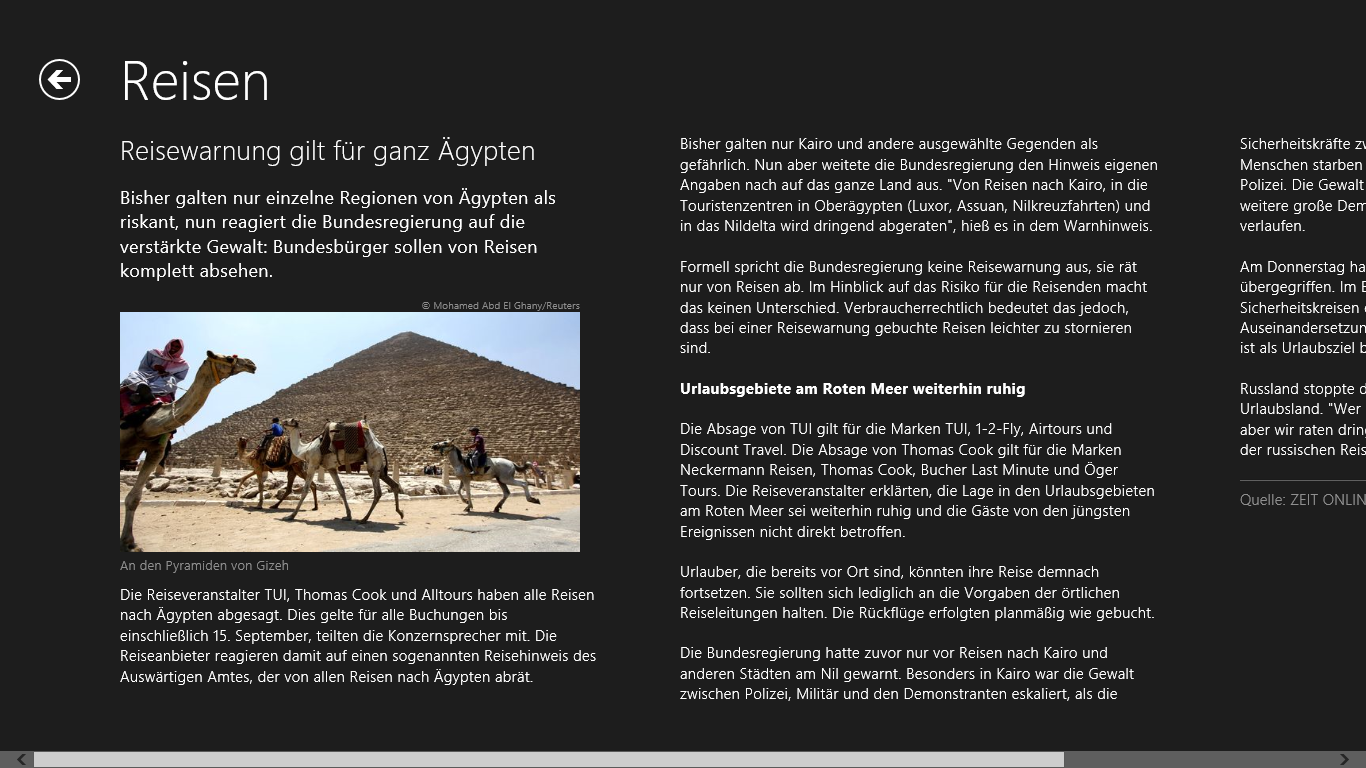
\includegraphics[width=\textwidth]{Bilder/Screenshots/app/reise_aegypten_4d.png} 
	\caption{Die Artikelansicht.}
	\label{fig:artikelansicht}
\end{figure}

Listing \ref{lst:artikelinfos} zeigt das Einfügen von Titel, Teasertext und  dem Bild. Anschließend fehlt noch der Artikeltext, die Quelle und der Autor. Um diese Daten zu bekommen und zu speichern ist ein weiterer \ac{xhr} nötig. Der \ac{xhr} wird mit der Artikel-URL aufgerufen, welche in jedem Teaserelement gespeichert ist. Auf diese Weise bekommt man das \ac{xml} der Artikel, wie es auch von der Webseite verwendet wird. Beim Parsen des Artikel-\ac{xml}s müssen drei Dinge besonders beachtet werden.

\begin{minipage}{\linewidth}
\begin{lstlisting}[language= Javascript,caption=Das Einfügen von Titel sowie Teasertext und Bild., label={lst:artikelinfos}]
element.querySelector("article .item-title").textContent = item.title;
element.querySelector("article .item-subtitle").innerHTML= item.teaserText;
element.querySelector("article .item-image").src = item.backgroundImage;
\end{lstlisting}   
\end{minipage}

Die Absätze des Artikels liegen in Paragraphen-Tags (<p></p>) vor. Es kann vorkommen, das außer dem reinen Text, zusätzlich noch Infoboxen im Artikel vorhanden sind. Ebenso ist es möglich, dass Nachrichten vom Mikroblogging Dienst Twitter eingebunden werden. Diese Abschnitte arbeiten ebenfalls mit Paragraphen-Tags. Da Infoboxen und Twitternachrichten sich inhaltlich nicht direkt in den Artikeltext eingliedern, müssen diese Abschnitte vorher herausgefiltert werden. Des weiteren sind in den meisten Artikeln auf der ZEIT ONLINE Webseite Hyperlinks, entweder auf andere Artikel oder auch andere Webseiten, vorhanden. Diese sind genau wie Infoboxen und Twitternachrichten unerwünscht, da sie, wenn sie vom User aufgerufen werden, in einer andere App (Internet Explorer) geöffnet werden würden. Dies unterbricht und stört das App-Erlebnis. Es muss dementsprechend darauf geachtet werden, dass nur der reine Artikeltext als Artikel gespeichert wird. Listing \ref{lst:artikelabsätze} verdeutlicht wie dies passiert. In Zeile 3 werden die Infoboxen und die Twitternachrichten herausgefiltert und in den Zeilen 8-13 werden die \textit{<a></a>} Tags mit Hilfe regulärer Ausdrücke gelöscht. Sobald der Artikel komplett geladen ist, wird er analog zu Listing \ref{lst:artikelinfos} in das \ac{html} Markup eingefügt.

\begin{minipage}{\linewidth}
\begin{lstlisting}[language= Javascript,caption=Vermeidung von Infoboxen \, Twitternachrichten und Hyperlinks in den Artikeln., label={lst:artikelabsätze}]
for (var n = 0; n < paragraphs.length; n++) {
    //exclude info box and tweets paragraphs
    if (paragraphs[n].parentNode.parentNode.parentNode.parentNode.nodeName != "infobox" && paragraphs[n].parentNode.getAttribute("class") != "twitter-tweet"){
        var xmlText = new XMLSerializer().serializeToString(paragraphs[n]);
        if (paragraphs[n].querySelector("a") != null) {
            var numberOfLinks = paragraphs[n].querySelectorAll("a").length;
            //remove hyperlinks
            for (var i = 0; i < numberOfLinks; i++) {
                var rx = new RegExp("<a[^<>]+>", "i");
                xmlText = xmlText.replace(rx, "");
                rx = new RegExp("</a>", "i");
                xmlText = xmlText.replace(rx, "");
            }
        }
        textContent = textContent + xmlText;
    }
}
\end{lstlisting}   
\end{minipage}

\subsection{Features}
\label{subsec:features}

\subsubsection{Artikeltitel ausblenden}
\label{subsubsec:artikeltitelausblenden}
Ein Hauptfeature der App ist es, dass in der Hubansicht und in der Ressortansicht die Artikeltitel ausgeblendet werden können und der User so nur noch eine Bilderwand vor sich hat. So kann er die Nachrichtenlage rein visuell erleben und erst wenn er auf einen Artikel klickt bekommt er im Artikel den Titel und Artikelinhalt zu sehen. Diese Funktion wird über eine Menüleiste am unteren Bildrand implementiert (siehe Abbildung \ref{fig:menubartitletoggle}). Um eine solche Menüleiste zu erzeugen genügt ein \textit{<div>} Container in der \textit{default.html} Datei mit einem \textit{data-win-control} Attribut, das den Wert \glqq WinJS.UI.AppBar\grqq\ bekommt. In diesem Element können anschließend \textit{<button>} Elemente angelegt werden. Diese sind später die sichtbaren Schaltflächen wenn die Menüleiste aufgerufen wird.

\begin{figure}[h]
	\centering
	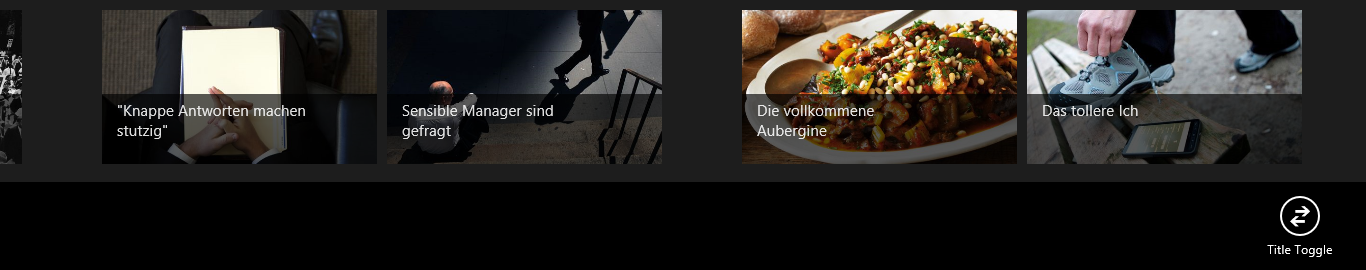
\includegraphics[width=\textwidth]{Bilder/Screenshots/app/title_toggle_menu_bar.png} 
	\caption{Untere Menüleiste mit der Funktion zum Artikeltitel ausschalten.}
	\label{fig:menubartitletoggle}
\end{figure}

In der Initialisierungsphase der App wird in der \textit{default.js} Datei der Click-Handler für den Button registriert. D.h. hier wird die Funktion angegeben, welche aufgerufen werden soll wenn der Button geklickt wird. In diesem Fall wird die Funktion \textit{titleToggle()} in der \textit{globals.js} Datei aufgerufen. In der \textit{globals.js} Datei befinden sich Variablen und Funktionen, die von mehreren Ansichten benutzt werden und deswegen global verfügbar sein sollen. Die \textit{titleToggle()} Funktion ist schließlich verantwortlich für das ausblenden der Artikeltitel.\\
Die Funktion sammelt dazu alle Elemente mit der Klasse \textit{item-overlay} in einem Array und setzt anschließend für alle gefundenen Elemente die CSS Eigenschft \textit{display} auf \glqq none\grqq\ . Das Resultat ist in Abbildung \ref{fig:ressortohnetitel} zu sehen.

\begin{figure}[h]
	\centering
	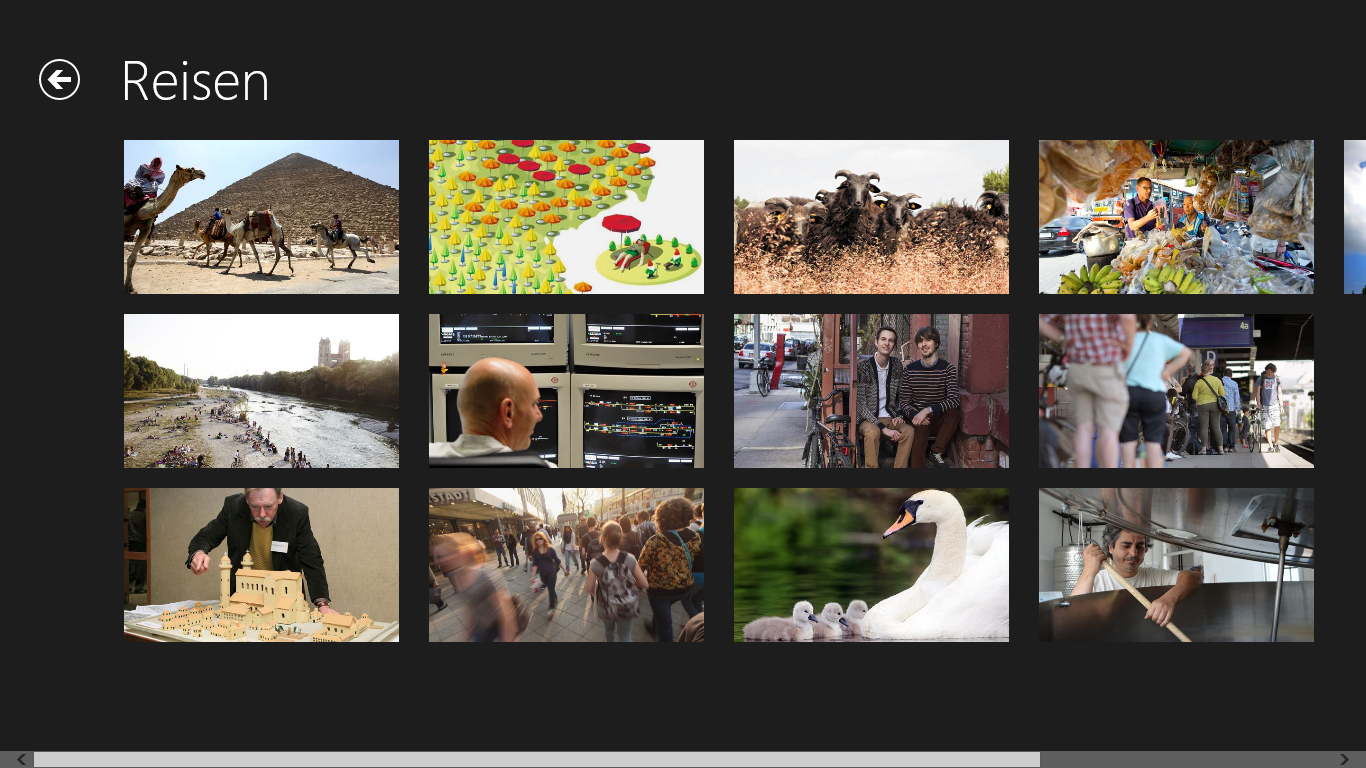
\includegraphics[width=\textwidth]{Bilder/Screenshots/app/reise_aegypten_3gdohne.png} 
	\caption{Das Reisen Ressort ohne Artikeltitel.}
	\label{fig:ressortohnetitel}
\end{figure}

\subsubsection{Schriftgröße verändern}
\label{subsubsec:schriftgroesseveraendern}
In der Artikelansicht hat der User die Möglichkeit, die Schriftgröße anzupassen. Es sind jeweils zwei Stufen größer, als auch zwei Stufen kleiner als die normale Größe möglich. Der  Ansatz ist grundsätzlich genau so wie bei der \glqq Titel-ausblenden\grqq\ Funktionalität. Zunächst wird ein Button in der unteren Menüleiste angelegt. Es wäre auch möglich zwei Buttons zu erstellen, einen für größer und einen für kleiner. Um die Entwicklungsmöglichkeiten jedoch weiter aus zu reizen gibt es in der App nur einen Button in der Menüleiste. Wird dieser geklickt erscheint noch ein weiteres Menü, ein sogenanntes \textit{Flyout-Menü}. In diesem sind schließlich die Schaltflächen für \glqq Schrift größer\grqq\ , \glqq Schrift kleiner\grqq\ und für \glqq Schriftgröße zurücksetzen\grqq\ . Ist die Schriftgröße z.B. auf der größten Stufe eingestellt, wird im Menü, der größer Button nicht mehr dargestellt. Abbildung \ref{fig:fontsizemenü} zeigt die verschiedenen Stati, die das Schriftgrößenmenü haben kann.

\begin{figure}[h]
	\centering
	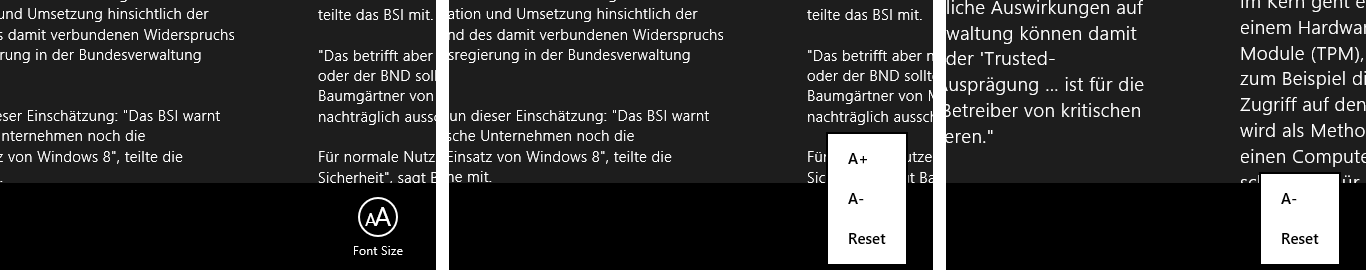
\includegraphics[width=\textwidth]{Bilder/Screenshots/app/font_size_menu_kompakt.png} 
	\caption{links: Schriftgröße Button im unteren Menü | mitte: Das Flyout-Menü mit allen Schaltflächen. | rechts: Das Flyout-Menü beim Aufruf wenn schon die größte Größe eingestellt ist.}
	\label{fig:fontsizemenü}
\end{figure} 

\subsubsection{Semantic Zoom}
\label{subsubsec:semanticzoom}
Das semantic Zoom Feature wird eingesetzt, wenn es in der Hubansicht sehr viele Bereiche gibt. Es soll dem User ermöglichen, ohne langes scrollen, zu den verschiedenen Bereichen in der Hubansicht zu springen. Beim Aufruf des semantic Zooms wird eine weitere Ebene über die Hubansicht gelegt. Typischer Weise werden in dieser Ebene nur die Verschiedenen Bereiche, ohne inhaltliche Elemente angezeigt. Bei ZEIGHT werden hier alle Ressorts mit dem jeweiligen Ressortnamen und einem zufälligen Bild aus dem Ressort angezeigt (siehe Abbildung \ref{fig:semanticzoom}). Diese Ansicht ist ebenfalls horizontal scrollbar, im direkten Vergleich zur Hubansicht jedoch viel kompakter und übersichtlicher. Klickt der User z.B. auf das Reisen Ressort, wird wieder zurück zur Hubansicht \glqq gezoomt\grqq. Der User hätte dann die Ansicht wie sie Abbildung \ref{fig:hubressortübersicht} auf Seite \pageref{fig:hubressortübersicht} zeigt. Das bedeutet es findet in beide Richtungen ein kontextsensitives Zoomen statt. Je nach dem wo sich der User in der Hubansciht befindet bzw. auf welches Ressort der User in der semantic Zoom Ebene klickt, wird an die entsprechende Stelle raus- bzw. reingezoomt.  

\begin{figure}[h]
	\centering
	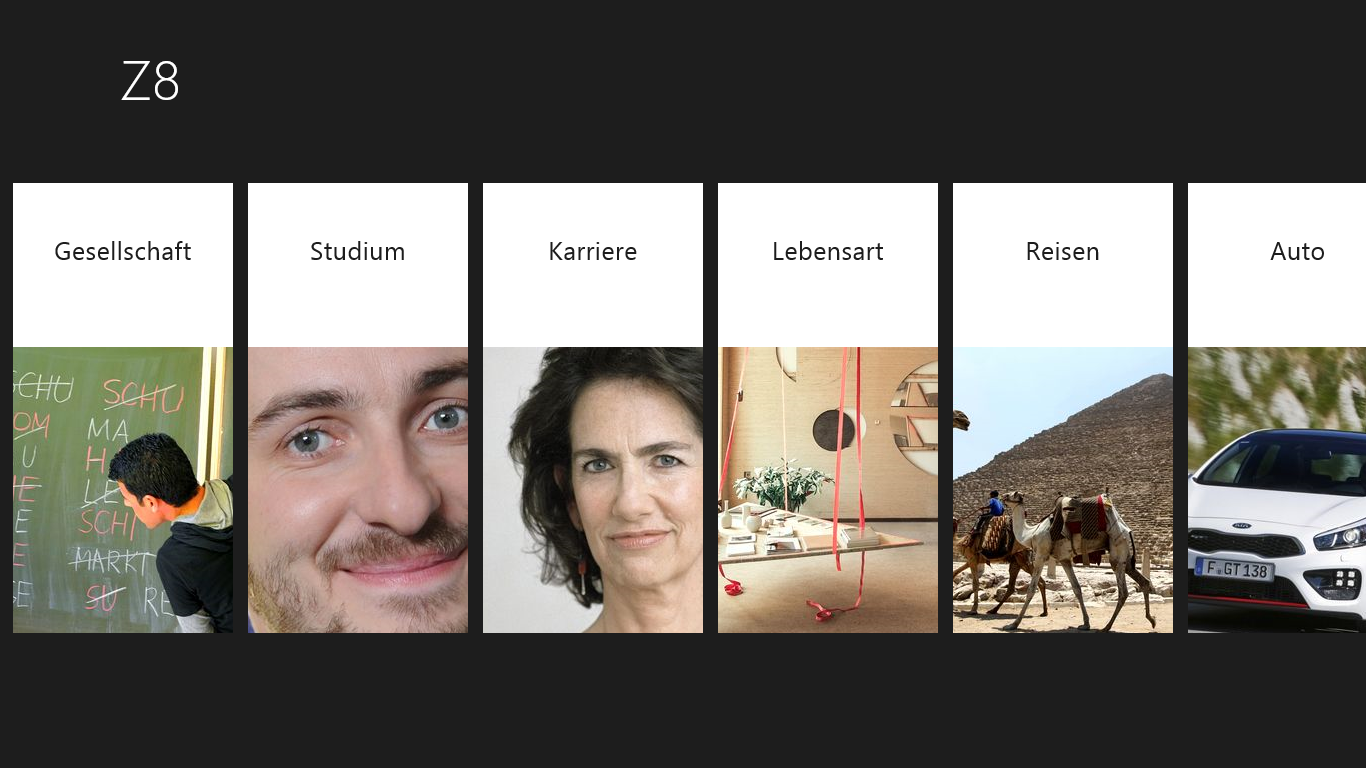
\includegraphics[width=\textwidth]{Bilder/Screenshots/app/reise_aegypten_1zoom.png} 
	\caption{Die semantic Zoom Ansicht.}
	\label{fig:semanticzoom}
\end{figure}  

Da der semantic Zoom von der Hubansicht aus aufgerufen wird und mit ihr interagiert, ist er dementsprechend in der \textit{groupedItems.html} und in der\textit{groupedItems.js} implementiert. Genau wie für die Hubansicht gibt es auch für den semantic Zoom ein Template für die einzelnen Elemente. Damit eine Interaktion zwischen der Hubansicht und dem semantic Zoom stattfinden kann, wird ein Wrapper \textit{div} Element um die \textit{WinJS.ListView} der Hubansicht und die \textit{WinJS.ListView} der semantic Zoom Ebene gezogen. Listing \ref{lst:semanticzoomwrapper} zeigt wie der Wrapper eingebunden ist. Das \textit{div} Element besitzt ein \textit{data-win-control} Attribut mit dem Wert \glqq WinJS.UI.SemanticZoom\grqq. Des weiteren kann der \textit{zoomFactor} und der initiale Zoomstatus festgelegt werden. Bei der ZEIGHT App ist dieser Zoomstatus initial auf false, da der User die Hubansicht als Einstiegspunkt in die App haben soll (nicht die semantic Zoom Ansicht).

\begin{minipage}{\linewidth}
\begin{lstlisting}[language= XML,caption=Der Semantic Zoom Wrapper., label={lst:semanticzoomwrapper}]
<div class="semanticZoom" data-win-control="WinJS.UI.SemanticZoom" data-win-options="{ zoomFactor: 0.5, initiallyZoomedOut: false }" style="height: 100%">
    <div class="groupeditemslist win-selectionstylefilled" aria-label="List of groups" data-win-control="WinJS.UI.ListView" data-win-options="{selectionMode: 'none'}"></div>
    <div class="groupeditemslistZoomOut groupeditemslist" aria-label="List of groups" data-win-control="WinJS.UI.ListView" data-win-options="{selectionMode: 'none'}"></div>
</div>
\end{lstlisting}   
\end{minipage}

\subsection{Entwicklungschronologie}
\label{subsec:entwicklungschronologie}


\newpage
\section{Evaluierung} 
\label{sec:evaluierung}
Bei der Evaluierung soll herausgefunden werden, inwieweit die App intuitiv benutzbar ist und ob ein alternativer Ansatz zum Konsumieren von Nachrichten Sinn macht und wie er ggf. funktionieren könnte. Es wird hierzu eine Art der Fokusgruppenevaluierung angewandt. Das bedeutet, es wird am Ende keine belastbaren statistischen Aussagen geben, sondern eher einen Trend zeichnen und einzelne Meinungen der Teilnehmer darstellen.

\subsection{Fokusgruppe}
\label{subsec:fokusgruppe}
Die Bezeichnung \glqq Fokusgruppe\grqq, die hier verwendet wird, steht in diesem Fall für eine kleine Gruppe von Testpersonen, im Gegensatz zu einer vollwertigen statistischen Auswertung. Es findet keine gemeinsame Diskussion statt, stattdessen muss jeder Teilnehmer einige Aufgaben ausführen und ein paar Fragen im Interview beantworten.


\begin{table}[h]
\centering
\begin{tabular}{|c|c|c|c|c|c|}
\hline 
\rule[-1ex]{0pt}{3.5ex} \textbf{Testperson (TP)} & \textbf{Beruf} & \textbf{Geschlecht} & \textbf{Alter} \\ 
\hline 
\rule[-1ex]{0pt}{2.5ex} 1 & Business Coach & W & 58 \\ 
\hline 
\rule[-1ex]{0pt}{2.5ex} 2 & Leiter Finanz- und Rechnungswesen & M & 58 \\ 
\hline 
\rule[-1ex]{0pt}{2.5ex} 3 & Student - Games Master & M & 27  \\ 
\hline 
\rule[-1ex]{0pt}{2.5ex} 4 & Wirtschaftspsychologin & W & • \\ 
\hline 
\rule[-1ex]{0pt}{2.5ex} 5 & Student - Games Master & M & 27 \\ 
\hline 
\end{tabular} 
\caption{Übersicht der Testpersonen.}
\label{tab:testpersonen}
\end{table}

Tabelle \ref{tab:testpersonen} zeigt die Übersicht der Testpersonen. Es wurde darauf geachtet, dass sich die Personen möglichst vom Beruf, Geschlecht und Alter her unterscheiden, um eine heterogene Gruppe zusammenzustellen und somit möglicherweise verschiedene Auffassungen und Herangehensweisen zu beobachten.


\subsection{Ablauf}
\label{subsec:ablauf}
Der Ablauf der Evaluierung setzt sich grob aus drei Abschnitten zusammen. Im ersten Teil soll überprüft werden inwieweit die Testpersonen, allein vom Betrachten des Teaserbilds eines Artikels, auf den groben, oder ggf. auch auf den genauen Inhalt des Artikels schließen können. Hierzu werden den Testpersonen zwei Ressorts in der Hubansicht, bei ausgeschalteten Titeln gezeigt. Zum einen, ein Das Politik-Ressort mit vorwiegend tagesaktuellen Nachrichten und zum anderen das Wissen-Ressort, welches auch zeitlose Artikel beinhalten kann. Abbildung \ref{fig:testbilder} zeigt die Bilder, welche die Testpersonen beurteilen sollten.

\begin{figure}[h]
	\centering
	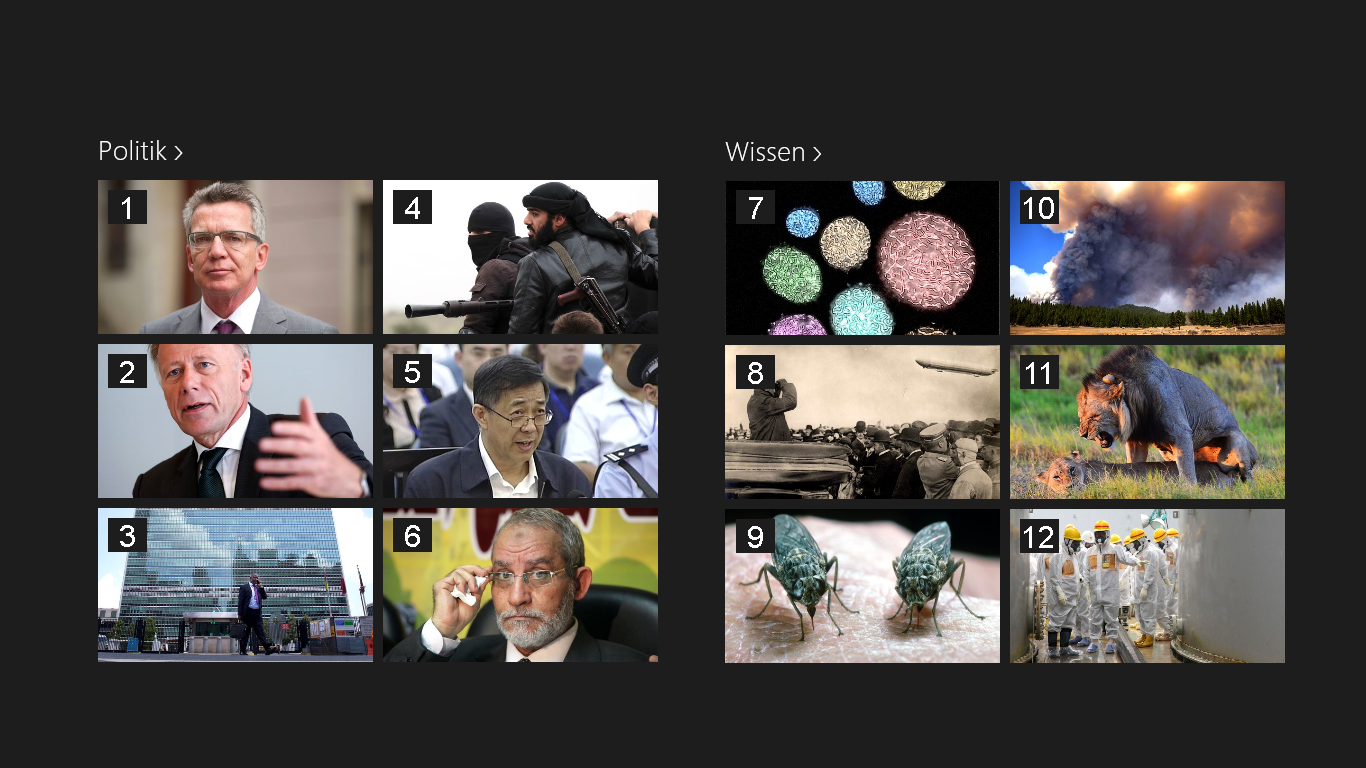
\includegraphics[width=\textwidth]{Evaluierung/Testbilder/collage_politik_wissen_numbers.png} 
	\caption{Die Testbilder aus dem Politik- und Wissen-Ressort.}
	\label{fig:testbilder}
\end{figure}  

Die Bilder sind nicht speziell zu diesem Zweck ausgewählt worden. Es handelt sich um die ersten sechs Artikel des jeweiligen Ressorts, wie sie am Sonntag den 25. August 2013 auch auf der ZEIT ONLINE Webseite zu finden waren. Die Testpersonen sollen jedes Bild einzeln durchgehen und zunächst eine Einschätzung zum groben Themengebiet geben und anschließend wenn möglich, so genau wie möglich beschreiben, um was es in dem jeweiligen Artikel gehen könnte. Die Ergebnisse werden in einem Tabellenkalkulationsprogramm festgehalten.\\

Im zweiten Teil der Evaluierung sollen die Testpersonen die App selber benutzen. Zum einen auf einem Notebook, auf welchem die App mit der Maus bedient wird und zum anderen auf dem \textit{Microsoft Surface}, ein Tablet, welches mit Touchgesten bedient wird. Es gibt vorher keine Instruktionen wie die App zu bedienen ist. Die Testpersonen sollen die App selbst entdecken und mögliche Features die programmiert wurden, finden und ausprobieren. Dies soll zeigen wie intuitiv das Navigationskonzept und die Menüführung der App sind.\\

Die Evaluierung endet mit dem dritten Teil, einem Interview. Hier sollen im Gespräch einige Fragen, zu den verschiedenen Teilen der Evaluierung beantwortet werden. Nachfolgend sind die groben Fragen aufgelistet, welche im Einzelfall durch Nachfragen leicht abgeändert werden können.

\begin{enumerate}
	\item Kannst du kurz deine bisherigen Erfahrungen mit Windows 8 schildern?
	\item In welcher Weise und wie oft konsumierst du Nachrichten im Allgemeinen? 
	\item Zu Teil 1: Wie war dein Gedankengang um herauszufinden was sich hinter den Bildern verbergen könnte?
	\item Zu Teil 2: Wie kamst du mit der App im Allgemeinen zurecht? War sie intuitiv? Welches Gerät hat dir besser gefallen und warum?
	\item Glaubst du der \glqq nur Bilder\grqq\ Modus macht neugierig? Oder glaubst du er hemmt den Nachrichtenkonsum? 
\end{enumerate}




\subsection{Ergebnisse}
\label{subsec:ergebnisse}
Hier sollen die Ergebnisse der Evaluierung dargestellt und bewertet werden. Zunächst geht es um die App und ihr Benutzungs- bzw. Navigationskonzept. Anschließend wird der Ansatz untersucht, ob Nachrichten auch auf eine andere Art und Weise konsumiert und entdeckt werden können.


\subsubsection{Intuitivität der App} 
\label{subsubsec:intuitivitätderapp}
Ob die App für die einzelne Testperson intuitiv bedienbar ist, hängt vermutlich direkt mit bereits gesammelten Windows 8 Erfahrungen zusammen. TP3-TP5 gaben bei der Frage nach der bisherigen Windows 8 Erfahrung an, bisher nur im Desktop-Modus von Windows 8 gearbeitet zu haben. Dies geschah ausschließlich mit Maus und Tastatur. TP1 hat bereits erste Erfahrungen mit der Modern UI Oberfläche gemacht. Außerdem ist sie vertraut mit dem Smartphonebetriebssystem von Microsoft, Windows Phone. TP2 hat bereits etwas tiefer gehende Erfahrungen mit Windows 8 und seinen Gesten, wenn auch hauptsächlich mit der Maus und weniger mit Touchbedienung.\\

TP1 fand das Navigationskonzept \glqq absolut intuitiv\grqq, wobei sie anmerkte, ihr hätte eine weitere Verbindung aus der Artikelansicht direkt zur Hubansicht gefallen. Klickt der User erst auf die Ressortübersicht und anschließend auf einen Artikel, kann nicht direkt zurück zur Hubansicht navigiert werden, sondern es muss der \glqq Umweg\grqq\ zurück über die Ressortübersicht genommen werden. TP2 meinte die App sei gut strukturiert, da diese Ebenenstruktur bekannt sei, merkte aber gleichzeitig an, das er sich vorstellen kann, das \textit{nicht} Windows 8 Nutzer zunächst Schwierigkeiten mit der Bedienung und Gesten haben könnten. TP3 und TP4 fanden es etwas verwirrend, dass im Artikel horizontal gescrollt wird, im Gegensatz zu normalen Webseiten. TP5 \glqq fehlte die nötige Vertrautheit mit der Modern UI Oberfläche\grqq\ um die nicht sofort sichbaren Bereiche der App (die Menüs) aufzurufen. Die Texte hingegen, seien sehr gut lesbar.\\

Generell lässt sich sagen, dass die Hauptnavigationsstruktur (Hubansicht, Ressortübersicht, Artikelansicht) von allen Testpersonen für intuitiv und gut verständlich empfunden wurde. Die meisten haben es auch geschafft die Menüs mit den Features (Titel ausblenden und Schriftgröße) aufzurufen. Ein Feature wurde allerdings nur von einer Testperson gefunden, der semantic Zoom. Das bedeutet, wenn dieses Navigationselement von einer App benutzt wird, sollte gezielt darauf hingewiesen werden, da die Möglichkeit eines semantic Zooms, gerade für Windows 8 Einsteiger, oft nicht sofort ersichtlich ist.

\subsubsection{Der nur Bilder Modus}
\label{subsubsec:nurbildermodus}
Hier sollen die Möglichkeiten und die Sinnhaftigkeit des \glqq nur Bilder\grqq Modus dargestellt und untersucht werden. Alle Testpersonen gaben an, täglich über verschiedenste Kanäle Nachrichten zu konsumieren. Sei es im Fernsehen, Online, Radio, Smartphone oder die Zeitung. Das bedeutet, es ist zu vermuten, dass alle Testpersonen über ein gewisses Basiswissen, was tagesaktuelle Geschehnisse betrifft, verfügen.\\
Im ersten Teil der Evaluation, sollten die Testpersonen versuchen herauszufinden, welcher Inhalt sich hinter den Teaserbildern von Abbildung \ref{fig:testbilder} verbergen könnte. Hierzu sollte zunächst ein grobes Themengebiet genannt werden und anschließend so genau wie möglich versucht werden, herauszufinden, worum es in dem jeweiligen Artikel geht. Ein Bild wurde in diesem Fall als \textit{genau} akzeptiert, wenn die Testperson nach dem obersten Themengebiet noch eine Stufe tiefer gehen konnte. So wurde es z.B. als richtig akzeptiert, wenn die Testperson bei Bild 10 nicht nur das grobe Thema \glqq Waldbrände\grqq, sondern auch \glqq San Francisco\grqq\ oder \glqq Yosemite Nationalpark\grqq\ richtig benannt hatte. Nach diesem Bewertungsschema wurden von den 12 Bildern im Durchschnitt 78,3\% grob, und 35\% auch genauer richtig zugeordnet. Das am häufigsten richtig zugeordnete Bild, ist Bild 10. Es wurde von allen Testpersonen grob als auch genau richtig erkannt. Dicht gefolgt Bild 5, welches alle Testpersonen grob, sowie 4 Testpersonen genauer richtig zuordnen konnten. Am wenigsten wurde Bild 3 erkannt. Es wurde nur von einer Testperson erkannt, dafür aber auch genau. Es geht in diesem Bild um die NSA-Affäre und den UN-Sicherheitsrat.\\
Die Testpersonen wurden im Interview gefragt, wie sie an diese Aufgabe herangegangen sind. In einem Punkt waren sich alle Testpersonen einig. Wenn man z.B. eine Person erkennt, muss man über andere Nachrichtenkanäle schon vorher etwas über diese Person gehört haben um den Inhalt genauer zuordnen zu können. TP1 meint, bei Bild 1 sei es sehr schwer etwas genaues sagen zu können, da diese Person zu verschiedenen Themen in Frage kommt. TP5 sagt zu Bild 6: \glqq Bei Bildern auf denen keine öffentlichen Personen drauf waren, hab ich einfach versucht über Vorurteile die Personen zu lesen\grqq. \\
Bei den Bildern aus dem Politik-Ressort wurde sich sehr auf das bereits aus anderen Nachrichtenquellen gehörte verlassen, wogegen bei den eher zeitlosen Artikeln und Bildern wie z.B. Bild 8 und Bild 11 die grobe Zuordnung recht leicht fiel, aber das Bild für die genaue Bestimmung nicht genügend Informationen lieferte und die Testpersonen auch nicht mit tagesaktuellem Wissen versuchen konnten zu raten. Bei Bild 8 geht es z.B. darum, dass Graf Zeppelin angeblich gar nicht der Erfinder des Zeppelins war und bei Bild 11 lautet der Titel: \glqq Hat nur der Mensch Sex in der Missionarsstellung?\grqq. \\

Es bleibt noch zu klären ob ein solcher Modus sinnvoll ist und inwieweit der User durch den \textit{nur Bilder} Modus neugierig gemacht wird oder ob er ihn eher in seinem Nachrichtenkonsumfluss stört und hemmt. TP sagt dazu: \glqq Das kommt drauf an was ich gerade möchte, [...] wenn ich mich kurz und prägnant informieren möchte  [...] muss unbedingt der Text drin sein, [aber] wenn ich mal ein bisschen Zeit habe und sitze irgendwo und warte, dann ist es eher der Entdeckermodus\grqq. TP2 meint, es hänge von der Veranlagung der Person ab. Es sei eine offene Herangehensweise nötig: \glqq Ich gucke mal was mir angeboten wird\grqq. Weiterhin glaubt TP2, dass Inhalte so eventuell besser im Gedächtnis bleiben, weil der User auf diese Weise aktiv auf ein Bild, welches seine Neugier geweckt hat, klickt und sich damit den Inhalt gewissermaßen selbst \glqq erarbeitet\grqq\ hat. TP4 sieht es ähnlich wie TP1. Es komme auf die Situation an und das Ziel des Nachrichtenkonsums an. TP5 meint, es hänge auch sehr stark vom jeweiligen Bild ab: \glqq Es muss eine klare Verbindung zum Inhalt geben [,um die Neugier zu wecken,] was bei reinen Personenbildern nicht der fall ist.\grqq. \\

Die Testpersonen stimmen bei dieser Frage grundlegend überein. Wenn der User gezielt tagesaktuelle Nachrichten konsumieren will, ist ein \textit{nur Bilder} Modus nicht zielführend. Es muss zu viel geraten und vermutet werden und im Zweifel klickt der User auf ein Bild und hat etwas ganz anderes erwartet und hat auf diese Weise ein negativ Erlebnis und ist genervt. Hat der User andererseits ein bisschen mehr Zeit und möchte mal etwas neues ausprobieren, sich durch die Nachrichtenwelt treiben lassen, dann stellt der \textit{nur Bilder} Modus eine interessante alternative dar. Hier kann sich der User ganz auf seinen Neugier- und Entdeckertrieb verlassen und das anklicken, wo er vielleicht schon etwas vermutet und er wissen möchte ob er richtig liegt. Der Trend zeigt deutlich, um den \textit{nur Bilder} Modus genießen zu können, sollte der User etwas Zeit mitbringen und sich bewusst darauf einlassen, nicht auf den ersten Blick alle Informationen dargelegt zu bekommen, sondern sich von der Neugier leiten zu lassen und es aktiv herauszufinden. 



\newpage
\section{Fazit}
\label{sec:fazit}

\newpage
\begin{singlespace}
	\bibliographystyle{natdin}
	\bibliography{ba_literatur}
\end{singlespace}

\newpage
\appendix
\pagenumbering{roman}
\thispagestyle{plain}

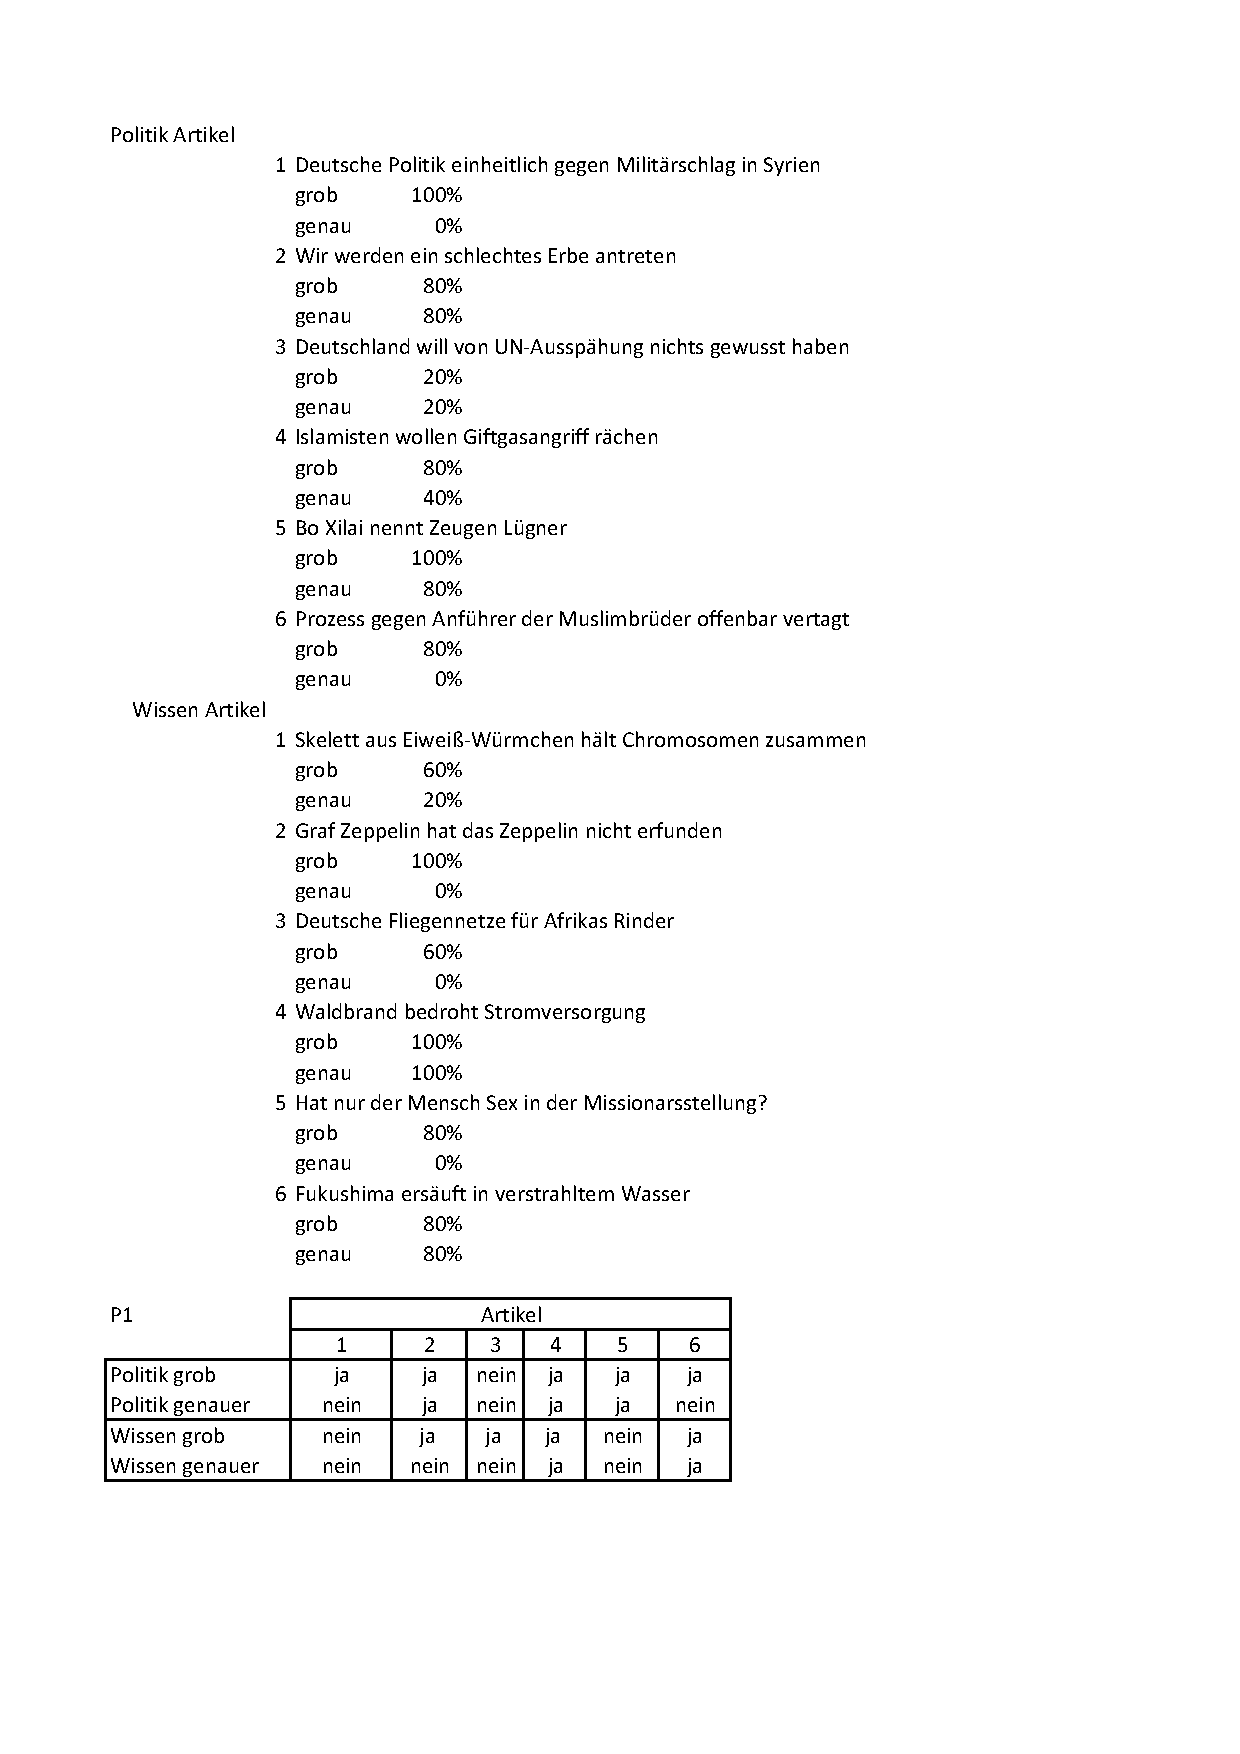
\includepdf[pages=1,scale=.9,pagecommand={\section{Detaillierte Evaluierung Bild-Inhalt Relation}}]{Evaluierung/rel_bilder_inhalt.pdf}
\includepdf[pages=2,scale=.9,pagecommand={}]{Evaluierung/rel_bilder_inhalt.pdf}

\end{document}